% last updated in April 2002 by Antje Endemann
% Based on CVPR 07 and LNCS, with modifications by DAF, AZ and elle, 2008 and AA, 2010, and CC, 2011; TT, 2014; AAS, 2016

\documentclass[runningheads]{llncs}
\usepackage{graphicx}
\usepackage{amsmath,amssymb} % define this before the line numbering.
% \usepackage{ruler}
\usepackage{color}
% \usepackage[width=122mm,left=12mm,paperwidth=146mm,height=193mm,top=12mm,paperheight=217mm]{geometry}

\usepackage{epsfig}
\usepackage{graphicx}
\usepackage{subfigure}
\usepackage{microtype}
\usepackage{multirow}
\usepackage{enumitem}
\usepackage{eso-pic}
\usepackage{bm}
\usepackage{booktabs}
\usepackage{adjustbox}
\usepackage{hyperref}

\begin{document}
% \renewcommand\thelinenumber{\color[rgb]{0.2,0.5,0.8}\normalfont\sffamily\scriptsize\arabic{linenumber}\color[rgb]{0,0,0}}
% \renewcommand\makeLineNumber {\hss\thelinenumber\ \hspace{6mm} \rlap{\hskip\textwidth\ \hspace{6.5mm}\thelinenumber}}
% \linenumbers
% \pagestyle{headings}
% \mainmatter
% \def\ECCV18SubNumber{547}  % Insert your submission number here

% \title{DU-Net: Densely Connected U-Nets for Human and Face Landmark Localization}
\title{Quantized Densely Connected U-Nets for Efficient Landmark Localization}

\titlerunning{Quantized Densely Connected U-Nets for Efficient Landmark Localization}
% Replace with a meaningful short version of your title
%
% \author{Zhiqiang Tang\inst{1} \and
% Xi Peng\inst{2} \and
% Shijie Geng\inst{1} \and Lingfei Wu\inst{3} \and Shaoting Zhang\inst{4} \and Dimitris N. Metaxas\inst{1}}
\author{Zhiqiang Tang$^1$ \and
Xi Peng$^2$ \and
Shijie Geng$^1$ \and Lingfei Wu$^3$ \and \\Shaoting Zhang$^4$ \and Dimitris Metaxas$^1$}
%
%Please write out author names in full in the paper, i.e. full given and family names. 
%If any authors have names that can be parsed into FirstName LastName in multiple ways, please include the correct parsing, in a comment to the volume editors:
%\index{Lastnames, Firstnames}
%(Do not uncomment it, because you may introduce extra index items if you do that, we will use scripts for introducing index entries...)
\authorrunning{Tang et al.}
% Replace with shorter version of the author list. If there are more authors than fits a line, please use A. Author et al.
%

% \institute{Rutgers University, NJ, USA\\ \email{\{zt53, sg1309, dnm\}@rutgers.edu}
% \and
% Binghamton University, NY, USA\\
% \email{xpeng@binghamton.edu}\\
% \and
% IBM T. J. Watson Research Center, NY, USA\\
% \email{lwu@email.wm.edu}
% \and
% University of North Carolina at Charlotte, NC, USA\\
% \email{rutgers.shaoting@gmail.com}}
\institute{
$^1$Rutgers University, 
\email{\{zt53, sg1309, dnm\}@rutgers.edu}\\
$^2$Binghamton University, \email{xpeng@binghamton.edu}\\
$^3$IBM T. J. Watson, 
\email{lwu@email.wm.edu}\\
$^4$SenseTime,
\email{zhangshaoting@sensetime.com}\\
}

%
\maketitle

\begin{abstract}

We propose a convolutional neural network (CNN) architecture for facial expression recognition. The proposed architecture is independent of any hand-crafted feature extraction and performs better than the earlier proposed convolutional neural network based approaches. We visualize the automatically extracted features which have been learned by the network in order to provide a better understanding. The standard datasets, i.e. Extended Cohn-Kanade (CKP) and MMI Facial Expression Databse are used for the quantitative evaluation. On the CKP set the current state of the art approach, using CNNs, achieves an accuracy of 99.2\%. For the MMI dataset, currently the best accuracy for emotion recognition is 93.33\%. The proposed architecture achieves $99.6$\% for CKP and $98.63$\% for MMI, therefore performing better than the state of the art using CNNs. Automatic facial expression recognition has a broad spectrum of applications such as human-computer interaction and safety systems. This is due to the fact that non-verbal cues are important forms of communication and play a pivotal role in interpersonal communication. The performance of the proposed architecture endorses the efficacy and reliable usage of the proposed work for real world applications.

\end{abstract}
\section{Introduction}

Locating visual landmarks, such as human body joints \cite{toshev2014deeppose} and facial key points \cite{xiong2013supervised}, is an important yet challenging problem. The stacked U-Nets, {\it e.g.} hourglasses (HGs) \cite{newell2016stacked}, are widely used in landmark localization. Generally speaking, their success can be attributed to design patterns: 1) within each U-Net, connect the top-down and bottom-up feature blocks to encourage gradient flow; and 2) stack multiple U-Nets in a cascade to refine prediction stage by stage.

However, the shortcut connection exists only ``locally'' inside each U-Net \cite{ronneberger2015u}. There is no ``global'' connection across U-Nets except the cascade. Blocks in different U-Nets cannot share features, which may impede the information flow and lead to redundant parameters.

We propose densely connected U-Nets (DU-Net) to address this issue. The key idea is to directly connect blocks of the same semantic meanings, {\it i.e.} having the same resolution in either top-down or bottom-up context, from any U-Net to all subsequent U-Nets. Please refer to Fig. \ref{fig:framework} for an illustration. The dense connectivity is similar to DenseNet \cite{huang2016densely} but generalizing the design philosophy from feature to semantic level. It encourages information flow as well as feature reuse ``globally'' across the stacked U-Nets, yielding improved localization accuracy. 

Yet there are critical issues in designing DU-Net: 1) The number of parameters would have a quadratic growth since $n$ stacked U-Nets could generate $O(n^2)$ connections. 2) A naive implementation may allocate new memory for every connection, making the training highly expensive and limiting the maximum depth of DU-Nets. 

% The training would be extremely memory expensive since a naive implementation has to make a copy of every connected feature for network forward and back propagation.  



\begin{figure*}[t!]
\centering
  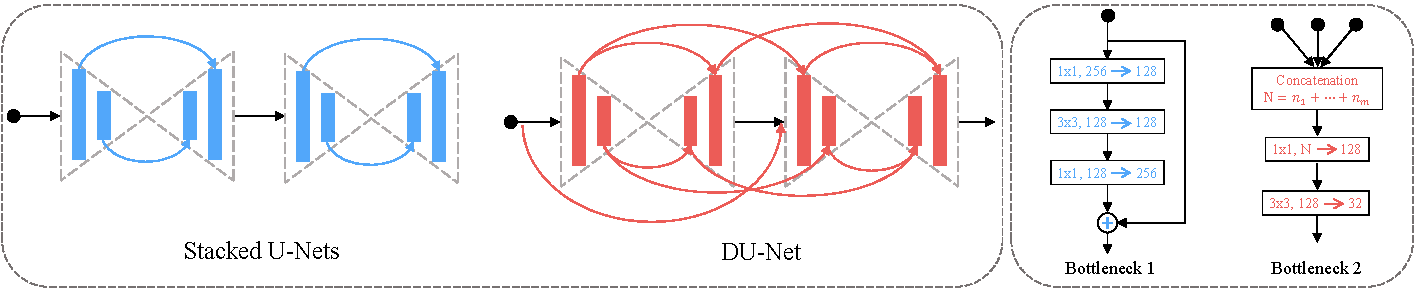
\includegraphics[width=1.0\linewidth]{figures/framework-cropped.pdf}
\caption{Illustration of stacked U-Nets and DU-Net. Stacked U-Nets has skip connections only within each U-Net. In contrast, DU-Net also connects blocks with the same semantic meanings across different U-Nets. The feature reuse could significantly reduce the size of bottleneck in each block, as shown in the right figure. Consequently, with the same number of U-Nets, DU-Net has only 30\% parameters of stacked U-Nets.}
\label{fig:framework}
\end{figure*}

% 
Our solution to those efficiency issues is threefold. {\bf First}, instead of connecting all stacked U-Nets, we only connect a U-Net to its $K$ successors. We name it as the $order$-$K$ connectivity, which aims to balance the fitting accuracy and parameter efficiency by cutting off long-distance connections. {\bf Second}, we employ a memory-efficient implementation in training. The key idea is to reuse a pre-allocated memory so all connected blocks could share the same memory. Compared with the naive implementation, this strategy makes it possible to train a very deep DU-Net (actually, $2\times$ deeper). {\bf Third}, to further improve the efficiency, we investigate an iterative design that may reduce the model size to one half. More specifically, the output of the first pass of the DU-Net is used as the input of the second pass, where detection or regression loss is applied as supervision. 

% %G%
% In view of deploying our approach on mobile devices, we further attempt to quantize weights, inputs, and gradients of DU-Net to low bit-width discrete values. This not only decreases the high precision operations but also shrinks the memory usage during training. By network quantization, the size of trained model can also be largely compressed.
% %G%
Besides shrinking the number of network parameters, we also study to further quantize each parameter. This motivates from the ubiquitous mobile applications. Although current mobile devices could carry models of dozens of MBs, deploying such networks requires high-end GPUs. However, quantized models could be accelerated by some specifically designed low-cost hardwares. Beyond only deploying models on mobile devices \cite{li2017deeprebirth}, training deep neural networks on distributed mobile devices emerges recently \cite{mcmahan2016communication}. To this end, we also try to quantize not only the model parameters but also its inputs (intermediate features) and gradients in training. This is the first attempt to investigate training landmark localizers using quantized inputs and gradients.


In summary, our key contributions are:
\begin{itemize}
    \item To the best of our knowledge, we are the first to propose quantized densely connected U-Nets for visual landmark localization, which largely improves the information flow and feature reuse at the semantic level.
    \item We propose the $order$-$K$ connectivity to balance accuracy and efficiency. It decreases the growth of model size from quadratic to linear by removing trivial connections. Experiments show it could reduce $\sim$70\% parameters of state-of-the-art landmark localizers.
    \item Very deep U-Nets can be trained using a memory-efficient implementation, where pre-allocated memory is reused by all connected blocks.
    \item We further investigate an iterative refinement that may cut down half of the model size, by forwarding DU-Net twice using either detection or regression supervision.
    %G%
    \item Different from previous efforts of quantizing only the model parameters, we are the first to quantize their inputs and gradients for better training efficiency on landmark localization tasks. By choosing appropriate quantization bit-widths for weights, inputs and gradients, quantized DU-Net achieves $\sim$75\% training memory saving with comparable performance. 
    %G%
    \item Exhaustive experiments are performed to validate DU-Net in different aspects. In both human pose estimation and face alignment, DU-Net demonstrates comparable localization accuracy and use $\sim$2\% model size compared with state-of-the-art methods.
\end{itemize}

% We are the first to deploy network quantization for better training efficiency on localization tasks. By choosing appropriate quantization bit-widths for weights, inputs and gradients, quantized DU-Net achieves at least 32$\times$ memory saving with comparable performance to the-state-of-art approaches. 


%The landmark localization such as human pose estimation \cite{toshev2014deeppose,newell2016stacked,wei2016convolutional}, facial landmark localization \cite{xiong2013supervised,zhang2014facial,sagonas2013300}, etc, plays an important role in the higher-level image understanding. The Convolutional Neural Networks (CNNs) have dominated this field, among which recent architecture of stacked hourglasses \cite{newell2016stacked}, a variant of the U-Net \cite{ronneberger2015unet}, becomes a standard solution. The skip connections between top-down and bottom-up blocks within a U-Net could preserve the spatial information and increase the gradient flow. With multiple U-Nets stacked together, the prediction could be refined stage by stage. However, the connections are only within each U-Net of the stacked hourglasses and no explicit connections exist between U-Nets, which may impede the information flow across them. And the blocks with the same semantics in different U-Nets cannot share features, leading to many redundant parameters. 

% Its success attributes to three key factors: repeated top-down, bottom-up inferences, intermediate supervisions and residual bottlenecks \cite{}. 

% The multiple stage top-down and bottom-up processing could better integrate both the local and global visual contexts into the final prediction. The intermediate supervision and residual bottlenecks, on the other hand, could alleviate the gradient vanish problem in deep networks.
%In this paper, we propose to densely connect stacked U-Nets by linking blocks with the same semantics in different U-Nets. We refer to this architecture as {\it Dense U-Nets}. The blocks in a U-Net could get direct inputs from its connected blocks in all preceding U-Nets, making the information flow more efficiently among the U-Nets. The feature reuse at each resolution could reduce the parameters in each block. The dense connectivity in our Dense U-Nets is different from that of DenseNet \cite{huang2016densely}. More specifically, layers only within each single block of the DenseNet are connected. In contrast, we connect blocks lying across the whole Dense U-Nets and connections of hierarchical blocks are mixed together. An illustration is given in Figure \ref{fig:framework}. We name it as the {\it global dense connectivity} to differentiate from the local one in the DenseNet.

% Besides, features in the Dense U-Nets are fused by the concatenation which could facilitate the information flow compared with the summation operation in the stacked hourglasses.

% Although the dense connectivity in our Dense U-Nets is similar with that of DenseNet \cite{}, 
% More recently, the DenseNet \cite{} achieves superior image classification performance over the ResNet \cite{} in terms of both the accuracy and model size, which benefits from the dense connections between layers. Its key insight is the feature reuse between layers of the same resolutions. The dense connectivity in the DenseNet, existing within one block, is local. By extending this principle, we propose a global dense connectivity, in contrast to the local connectivity in \cite{}, that blocks at the same locations of different U-Nets are connected. Hence, we refer to this architecture as {\it Dense U-Nets}. To our best knowledge, we are the first to generalize the local dense connectivity into the stacked U-Nets. 
% The global dense connectivity could make it easier to train much deeper stacked U-Nets.

% This motivates us to replace the residual modules  in the stacked hourglasses with the dense connected layers. However, this dense connectivity exists only locally within a contiguous  block in which all feature maps have the same spatial resolution. A U-Net, on the other hand, consists of a sequence of top-down and bottom-up blocks. A straight way is to turn each block into a dense block with multiple layers. However, this would sacrifice the spirit of stacked hourglasses that multiple stacked hourglasses outperform a single hourglass with multiple layers in each block.

% In order to integrate the structure of stacked U-Nets together with the idea of dense connectivity, we propose a global dense connectivity, in contrast to the local connectivity in \cite{}, that blocks at the same locations of different U-Nets are connected. Hence, we refer to this architecture as {\it Dense U-Nets}. The connected layers in the Dense U-Nets distribute along the whole network rather than in local continuous blocks. Compared with the local residual modules in the stacked hourglasses, the global dense connections could significantly facilitate the gradient to flow across stacked U-Nets.

%In practice, the Dense U-Nets have the efficiency problems of both parameter and training memory. First, suppose a Dense U-Nets contains $n$ U-Nets, there would be $O(n(n-1)/2)$ connections. Even though we use the dense bottleneck in Figure \ref{fig:framework}, the number of conv($1\times 1$) parameters still has the quadratic growth. Inspired from the Variable Order Markov (VOM) models \cite{begleiter2004prediction}, we propose the order-K connectivity that, instead of linking all the U-Nets, we connect only a fixed number of U-Nets. The goal is to use the minimum connections achieving the most obvious improvements. The multiple intermediate supervisions in the Dense U-Nets are good compensates for the order-K connectivity since they could provide additional gradients. The DenseNet does not have this advantage since it has only one supervision at the end.

% Furthermore, different from the DenseNet with only one supervision, the Dense U-Nets have multiple intermediate supervisions. The global dense connections plus the intermediate supervisions could bring faster convergence on the training set, but also gives rise to the concern of overfitting. Inspired from the Variable Order Markov (VOM) models \cite{}, we propose the order-K connectivity that, instead of linking all the U-Nets, we connect only a fixed number of U-Nets. The goal is to use the minimum connections achieving the most obvious improvement. Another advantage of order-K connectivity is that it has fewer parameters compared with the dense connectivity.

%Benefiting from the order-K connectivity, the Dense U-Nets could achieve comparable performance of stacked hourglasses with only one-third parameters. However, a naive implementation of the order-K connectivity could make the training very memory expensive. Therefore, we employ the memory efficient implementation \cite{pleiss2017memory}. The key idea is to share memories for time efficient operations such as concatenation and batch norm \cite{ioffe2015batch} within the connected layers. By pre-allocating a fixed memory, the later features produced by these operations would replace earlier features. So we need to re-compute those replaced features in the backward phase. The memory efficient implementation makes it possible to train Dense U-Nets two times deeper than the stacked hourglasses. 

%Furthermore, we also investigate to use the iterative refinement improving the parameter efficiency. Given a Dense U-Nets, we compare its performance with another Dense U-Nets with only half depth but an additional iteration. Besides, both detection and regression losses \cite{bulat2016human} were used in the landmark detection tasks, but there is no investigation yet about how they independently and collaboratively affect the prediction. We will give their detailed comparison in our experiments.

%In summary, the key contributions are:
%\begin{itemize}
%    \item To our best knowledge, we are the first to use the dense connectivity among the stacked U-Nets. The global dense connectivity in our Dense U-Nets is different from the local one in the DenseNet \cite{huang2016densely}.
%    \item We propose the order-K connectivity to make the Dense U-Nets parameter efficient. The order-K connectivity could decrease the growth of conv($1\times 1$) parameters from quadratic to linear. With comparable performance as the stacked hourglasses \cite{newell2016stacked}, it makes the Dense U-Nets require only one-third parameters. 
%    \item The memory efficient implementation of Dense U-Nets is provided to reduce its training memory usage. It makes it possible to train Dense U-Nets two times deeper than the stacked hourglasses.
%    \item We further explore using iterative refinement to improvement the parameter efficiency. At the same time, we investigate how different combinations of the detection and regression losses affect the performance.
%\end{itemize}
The majority of existing approaches to WSD formulate this task as  MIL. In this formulation an image is interpreted as a bag of regions. If the image is labeled as positive, then one of the regions is assume to tightly contain the object of interest. If the image is labeled as negative, then no region contains the object. Learning alternates between estimating a model of the object appearance and selecting which regions in the positive bags correspond to the object using the appearance model. 

The MIL strategy results in a non-convex optimization problem; in practice, solvers tend to get stuck in local optima such that the quality of the solution strongly depends on the initialization. Several papers have focused on developing various initialization strategies \cite{Kumar10a,Deselaers10,Song14a,Cinbis15} and on regularizing the optimization problem \cite{Song14,Bilen14}. Kumar~\etal \cite{Kumar10a} propose a self-paced learning strategy that progressively includes harder samples to a small set of initial ones at training. Deselaers~\etal~\cite{Deselaers10} initialize object locations based on the objectness score. Cinbis~\etal \cite{Cinbis15} propose a multi-fold split of the training data to escape local optima. Song~\etal~\cite{Song14} apply Nesterov's smoothing technique \cite{Nesterov05} to the latent SVM formulation \cite{Felzenszwalb10a} to be more robust against poor initializations. Bilen~\etal~\cite{Bilen14} propose a smoothed version of MIL that softly labels object instances instead of choosing the highest scoring ones. Additionally, their method regularizes the latent object locations by penalizing unlikely configurations based on symmetry and mutual exclusion principles.

Another line of research in WSD \cite{Song14,Song14a,Wang14a} is based on the idea of identifying the similarity between image parts. Song~\etal \cite{Song14} propose a discriminative graph-based algorithm that selects a subset of windows such that each window is connected to its nearest neighbors in positive images. In~\cite{Song14a}, the same authors extend this method to discover multiple co-occurring part configurations. Wang~\etal~\cite{Wang14a} propose an iterative technique that applies a latent semantic clustering via latent Semantic Analysis (pLSA) on the windows of positive samples and selects the most discriminative cluster for each class based on its classification performance. Bilen~\etal \cite{Bilen15} propose a formulation that jointly learns a discriminative model and enforces the similarity of the selected object regions via a discriminative convex clustering algorithm.

Recently a number of researchers \cite{Oquab14,Oquab15} have proposed weakly supervised localization principles to improve classification performance of CNNs without providing any annotation for the location of objects in images. Oquab~\etal \cite{Oquab14} employ a pre-trained CNN to compute a mid-level image representation for images of PASCAL VOC. In their follow-up work, Oquab~\etal \cite{Oquab15} modify a CNN architecture to \emph{coarsely} localize object instances in image while predicting its label. 

Jaderberg~\etal~\cite{Jaderberg15c} proposed a CNN architecture in which a subnetwork automatically pre-transforms an image in order to optimize the classification accuracy of a second subnetwork. This ``transformer network'', which is trained in an end-to-end fashion from image-level labels, is shown to align objects to a common reference frame, which is a proxy to detection. Our architecture contains a mechanism that pre-select image regions that are likely to contain the object, also trained in an end-to-end fashion; while this may seem very different, this mechanism can also be thought as learning transformations (as the ones that map the detected regions to a canonical reference frame). However, the nature of the selection process in in our and their networks are very different.

\begin{figure*}
\centering
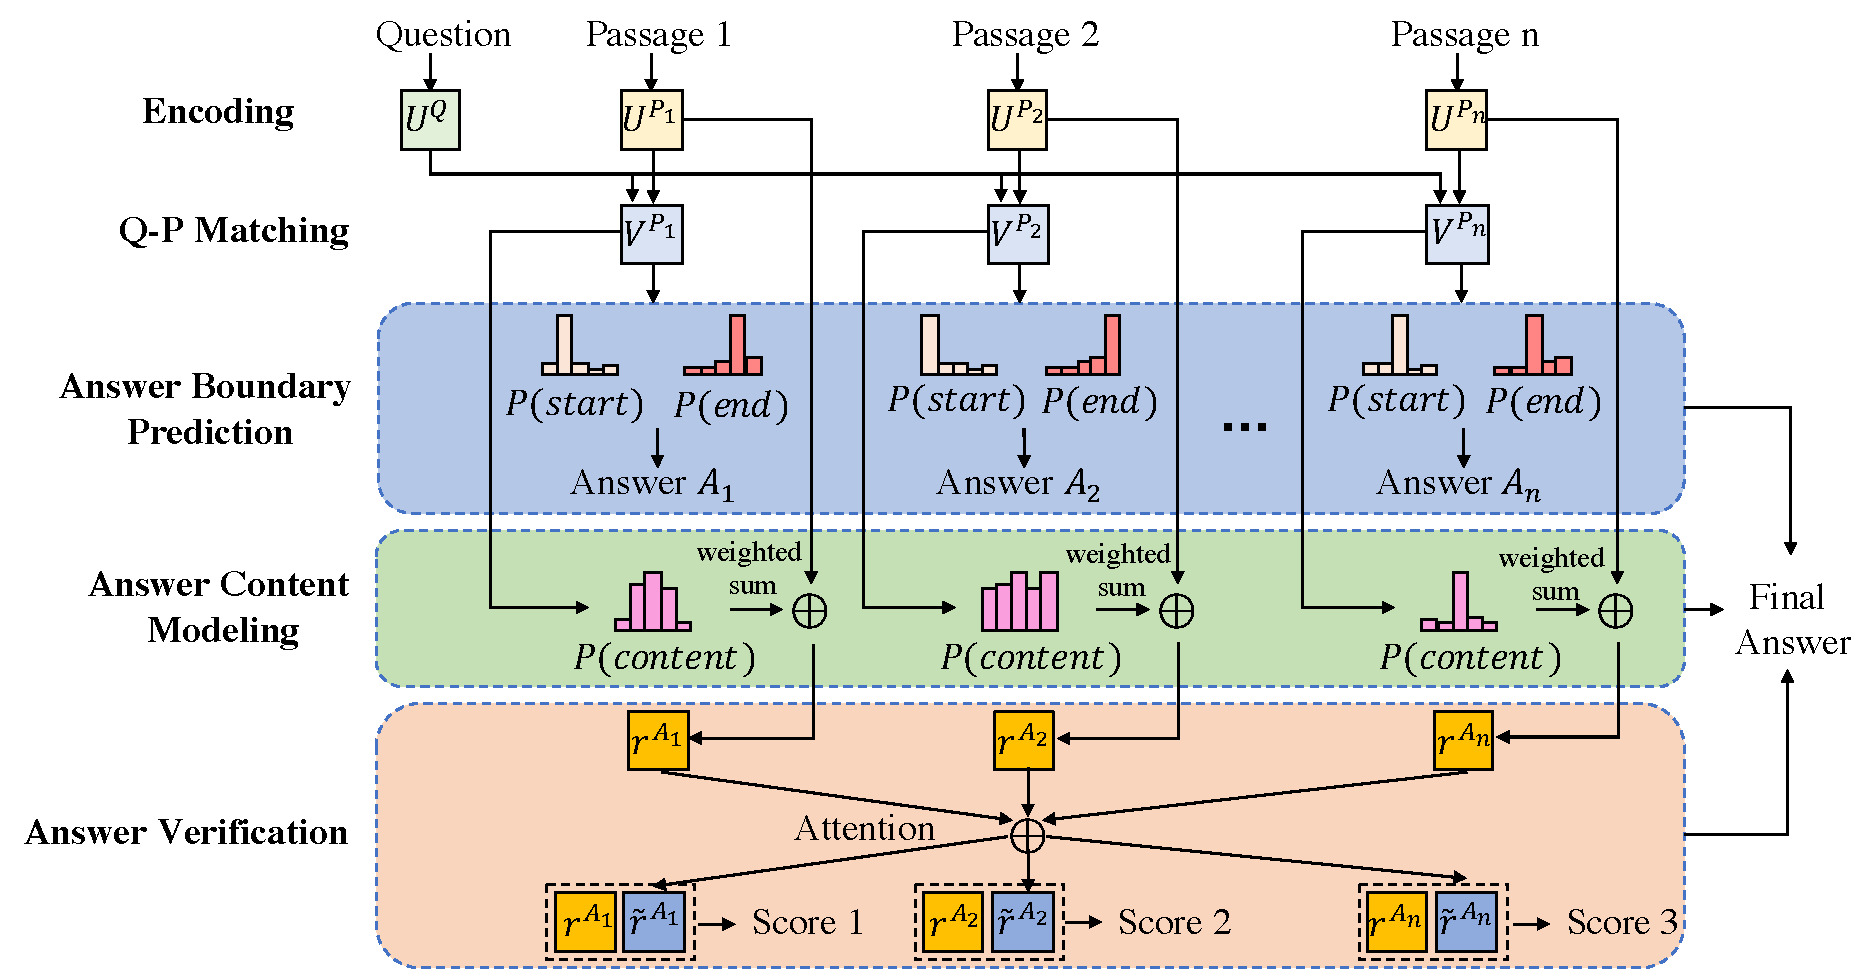
\includegraphics[width=0.85\textwidth]{architecture}
\caption{The overall architecture of our proposed network. The network
contains layers of symmetric convolution (encoder) and deconvolution (decoder).
Skip shortcuts are connected every a few (in our experiments, two) layers from
convolutional feature maps to their mirrored deconvolutional feature maps.
The response from a convolutional layer is directly propagated to the corresponding
mirrored deconvolutional layer, both forwardly and backwardly.}
\label{fig1}
\end{figure*}

\section{Very deep convolutional auto-encoder for image restoration}
\label{sec:main}

The proposed framework mainly contains a chain of convolutional layers and symmetric
deconvolutional layers, as shown in Figure \ref{fig1}. Skip connections are connected
symmetrically from convolutional layers to deconvolutional layers. We term our method
``RED-Net''---very deep Residual Encoder-Decoder Networks.


\subsection{Architecture}

The framework is fully convolutional (and deconvolutional.  Deconvolution is essentially unsampling convolution). Rectification layers are added
after each convolution and deconvolution. For low-level image restoration problems, we
use neither pooling nor unpooling in the network as usually pooling discards useful image
details that are essential for these tasks. It is worth mentioning that since the convolutional
and deconvolutional layers are symmetric, the network is essentially pixel-wise prediction,
thus the size of input image can be arbitrary. The input and output of the network are images
of the same size $w\times h\times c$, where $w$, $h$ and $c$ are width, height and number of channels.

Our main idea is that the convolutional layers act as a feature extractor, which preserve the
primary components of objects in the image and meanwhile eliminating the corruptions.
After forwarding through the convolutional layers, the corrupted input  image is converted into
a ``clean" one. The subtle details of the image contents may be lost during this process.
The deconvolutional layers are then combined to recover the details of image contents.
The output of the deconvolutional layers is the recovered clean version of the input image.
Moreover, we add skip connections  from a convolutional layer to its corresponding
mirrored deconvolutional layer. The passed convolutional feature maps are summed to the
deconvolutional feature maps element-wise, and passed to the next layer after rectification.
Deriving from the above architecture, we have used two networksvin our experiments, which are of 20 layers
 and 30 layers
respectively, for image denoising, image super-resolution, JPEG deblocking and image inpainting.



\subsection{Deconvolution decoder}

Architectures combining layers of convolution and deconvolution~\cite{DBLP:conf/iccv/NohHH15,
hong2015decoupled} have been proposed for semantic segmentation recently. In contrast to
convolutional layers, in which multiple input activations within a filter window are fused
to output a single activation, deconvolutional layers associate a single input activation with
multiple outputs. Deconvolution is usually used as {\em learnable up-sampling layers}.

 In our network,
the convolutional layers successively down-sample the input image content into a  small
size abstraction. Deconvolutional layers then up-sample the abstraction back into its original resolution.

Besides the use of skip connections, a main difference between our model and
~\cite{DBLP:conf/iccv/NohHH15,hong2015decoupled} is that our network is fully convolutional and
deconvolutional, i.e., without pooling and un-pooling. The reason is that for low-level image restoration,
the aim is to eliminate low level corruption while preserving image details instead of learning
image abstractions. Different from high-level applications such as segmentation or recognition,
pooling typically eliminates the abundant image details and can deteriorate restoration performance.



One can simply replace deconvolution with convolution, which results in an architecture that is
very similar to recently proposed very deep fully convolutional neural networks
~\cite{DBLP:conf/cvpr/LongSD15,DBLP:journals/pami/DongLHT16}. However, there exist essential
differences between a fully convolution model and our model. Take image denoising as an example.
We compare the 5-layer and 10-layer fully convolutional network with our network
(combining convolution and deconvolution, but without skip connection). For fully convolutional
networks, we use padding or up-sampling the input to make the input and output be of the same size.
For our network, the first 5 layers are convolutional and the second 5 layers are deconvolutional.
All the other parameters for training are identical, i.e., trained with SGD and learning rate of
$10^{-6}$, noise level $\sigma=70$. The Peak Signal-to-Noise Ratio (PSNR) on the validation set
is reported, which shows that using deconvolution works better than the fully convolutional
counterpart, as shown in Figure \ref{fig2}.


Furthermore, in Figure \ref{fig3}, we visualize some results that are outputs of layer 2, 5, 8 and 10
from the 10-layer fully convolutional network and ours. In the fully convolution case, the noise
is eliminated step by step, i.e., the noise level is reduced after each layer. During this process,
the details of the image content may be lost. Nevertheless, in our network, convolution  preserves
the primary image content. Then deconvolution is used to compensate the details.


\begin{figure}[htb!]
\centering
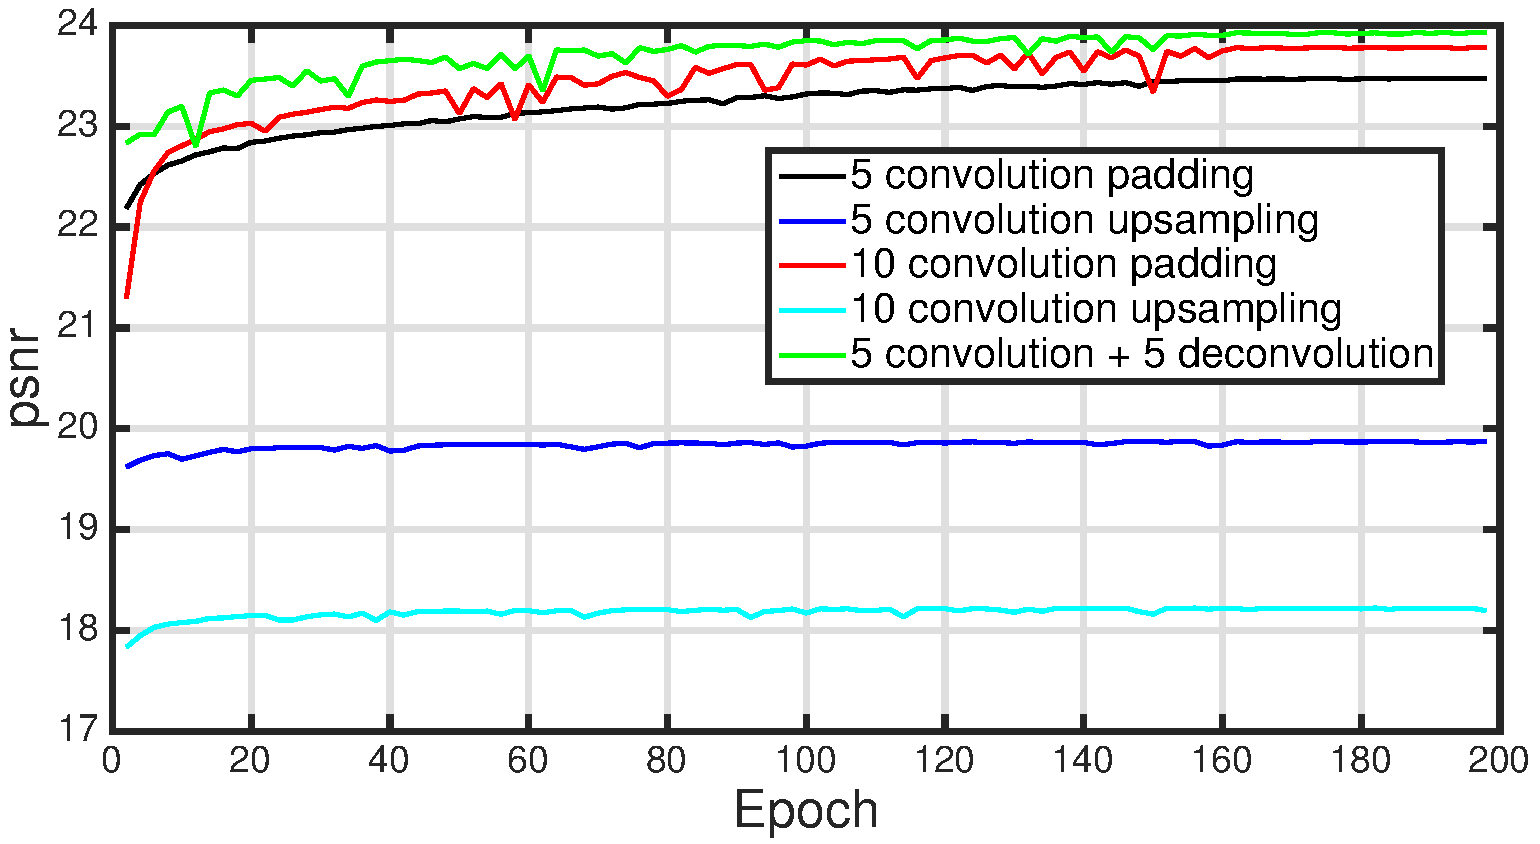
\includegraphics[width=0.48\textwidth]{conv-vs-decv}
\caption{ PSNR  values  on the validation set during training. Our model  exhibits better PSNR
than the compared ones upon convergence.}
\label{fig2}
\end{figure}



\begin{figure}[htb!]
\centering
\subfigure[]{ 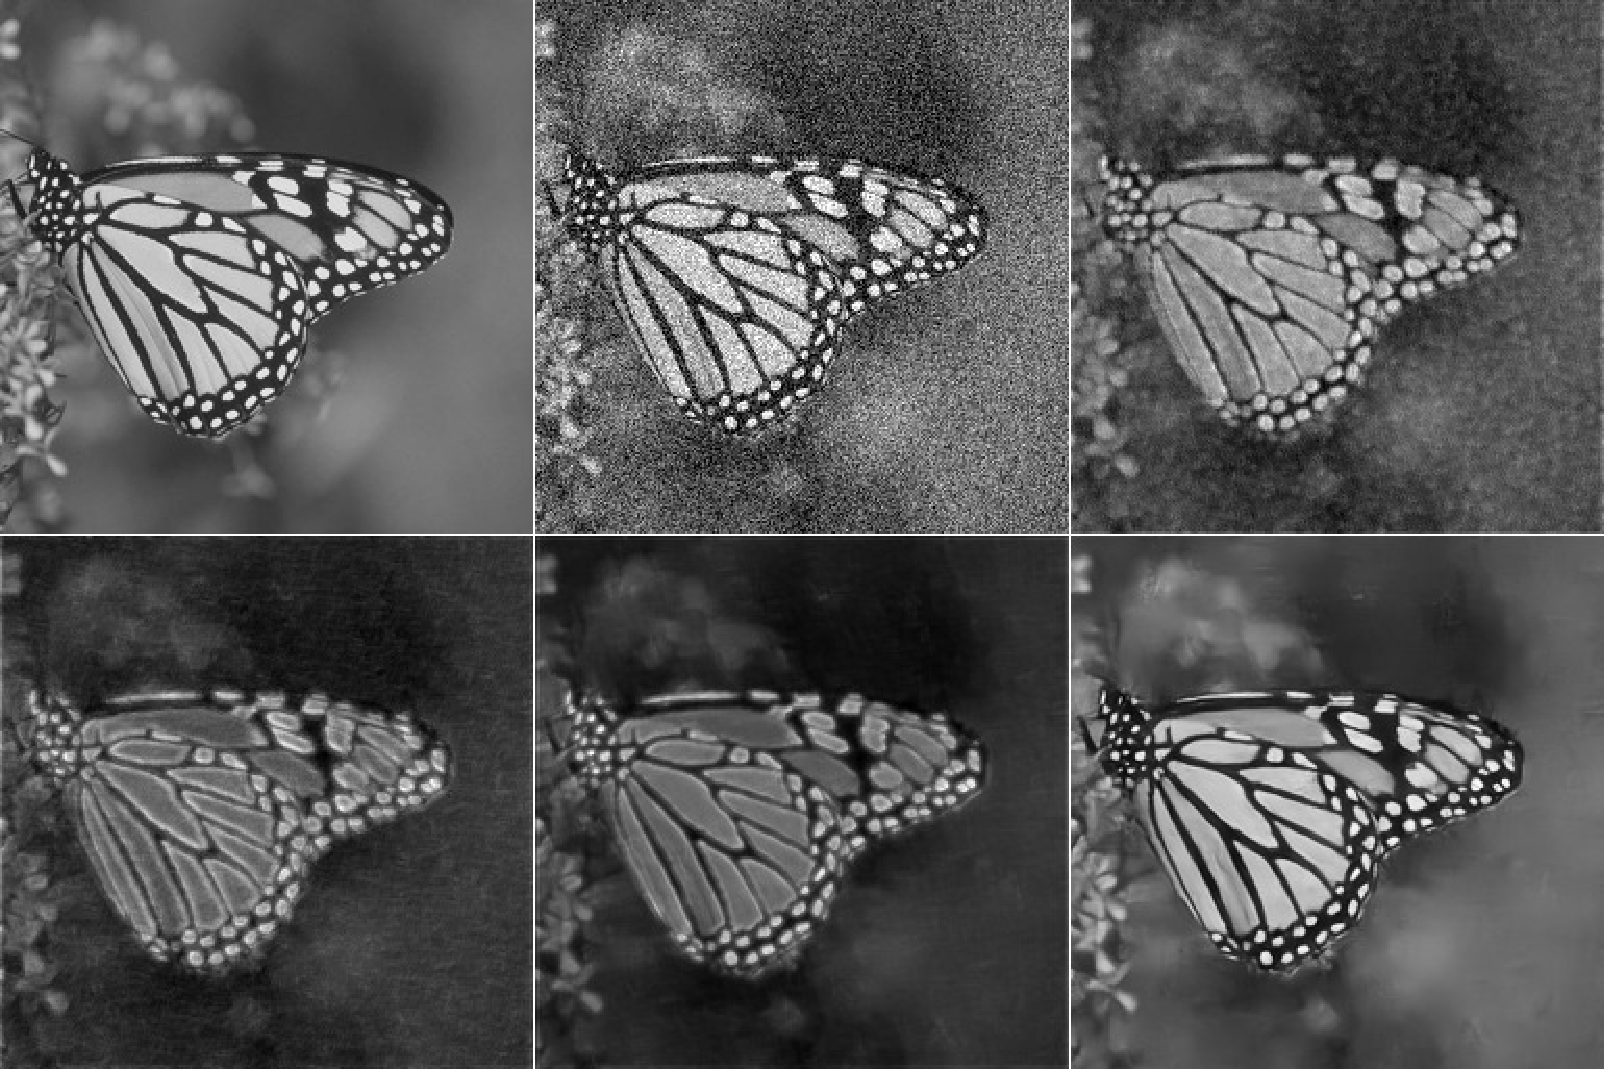
\includegraphics[width=0.48\textwidth]{show-denoising-conv} }
\subfigure[]{ 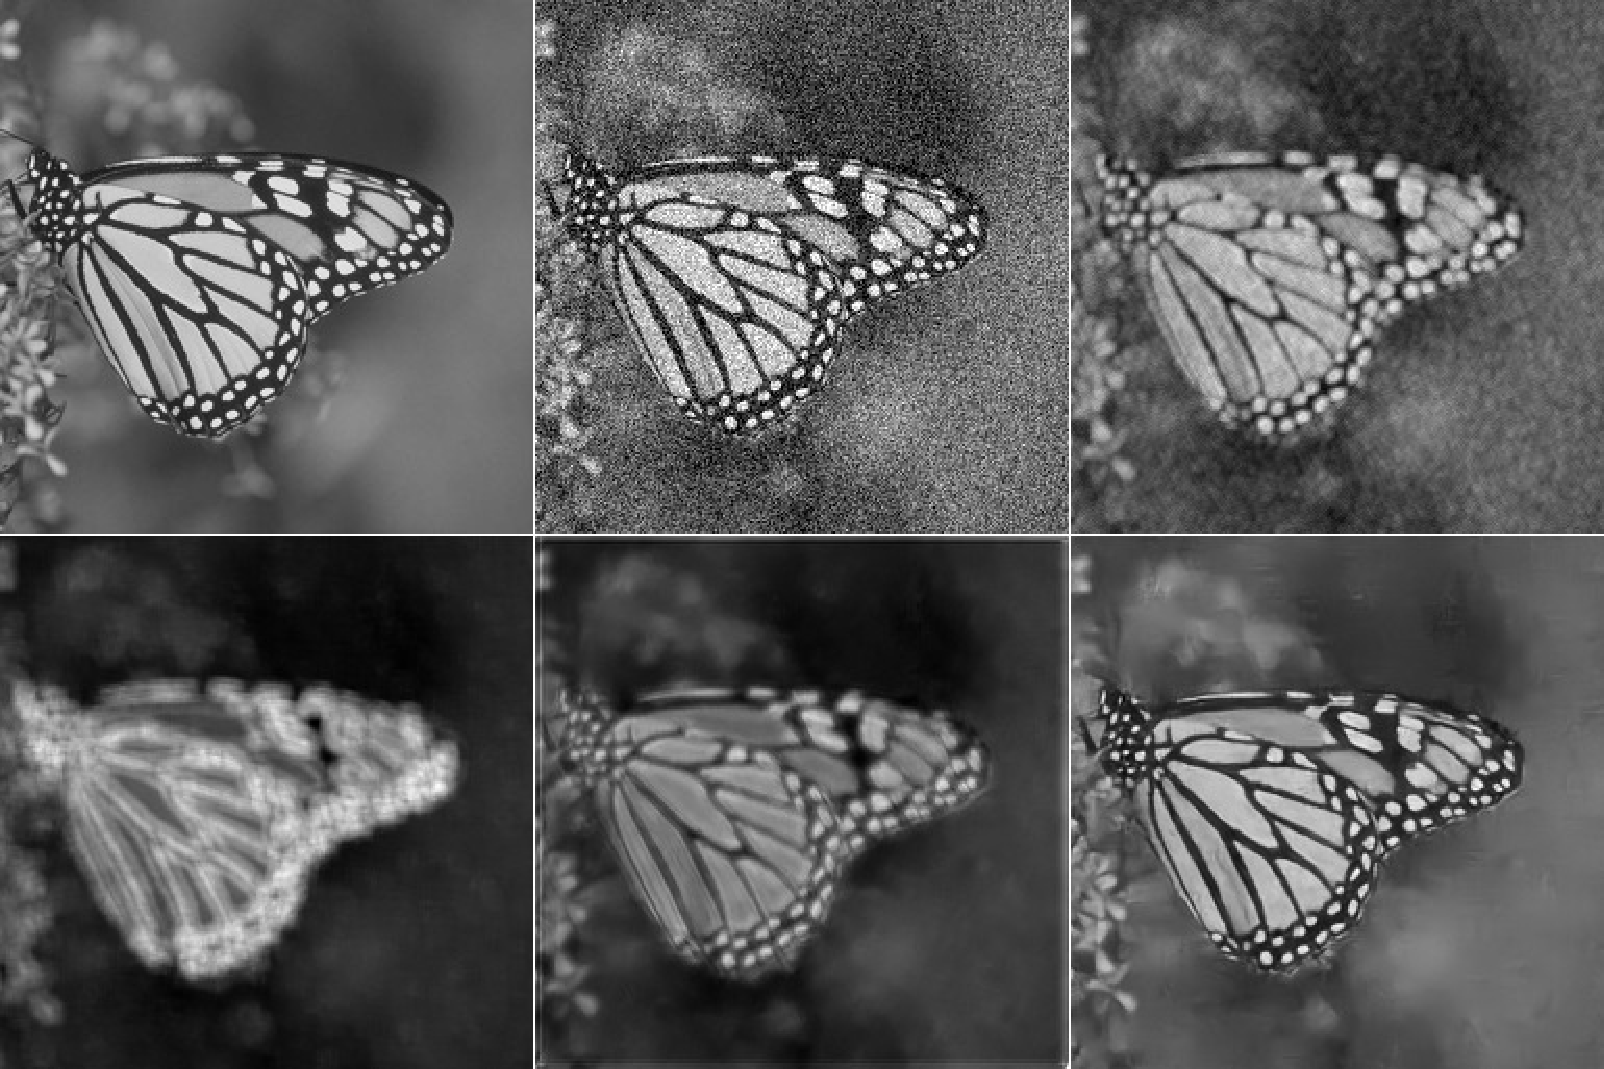
\includegraphics[width=0.48\textwidth]{show-denoising-decv} }
\caption{ (a) Visualization of the 10-layer fully convolutional network. The images from
top-left to bottom-right are: clean image, noisy image, output of conv-2, output of conv-5,
output of conv-8 and output of conv-10, where ``conv-$i$" stands for the $i$-th convolutional layer;
(b) Visualization of the 10-layer convolutional and deconvolutional network. The images from
top-left to bottom-right are: clean image, noisy image, output of conv-2, output of conv-5,
output of deconv-3 and output of deconv-5, where ``deconv-$i$" stands for the $i$-th deconvolutional layer.}
\label{fig3}
\end{figure}




\subsection{Skip connections}

An intuitive question is that, is a network with deconvolution able to recover image details from
the image abstraction only? We find that in shallow networks with only a few layers
of convolution layers, deconvolution is able to recover the details. However, when the
network goes deeper or using operations such as max pooling, even with deconvolution layers, it does not work
that well, possibly because too much details are already lost in the convolution and pooling.


The second question is that, when our network goes deeper, does it achieve performance gain?
We observe that deeper networks in image restoration tasks tend to easily suffer from
performance degradation. The reason may be two folds. First of all, with more layers of
convolution, a significant amount of image details could be lost or corrupted. Given only the image abstraction,
recovering its details is an under-determined problem. Secondly, in terms of optimization,
deep networks often suffer from gradients vanishing and become much harder to train---a problem
that is well addressed in the literature of neural networks.


To address the above two problems, inspired by highway networks \cite{DBLP:journals/corr/SrivastavaGS15}
and deep residual networks \cite{DBLP:journals/corr/HeZRS15}, we add skip connections between
two corresponding convolutional and deconvolutional layers as shown in Figure \ref{fig1}.
A building block is shown in Figure \ref{fig4}. There are two reasons for using such connections.
First, when the network goes deeper, as mentioned above, image details can be lost, making deconvolution
weaker in recovering them. However, the feature maps passed by skip connections carry much image detail,
which helps deconvolution to recover an improved clean version of the image. Second, the skip connections also achieve
benefits on back-propagating the gradient to bottom layers, which makes training deeper network much
easier as observed in \cite{DBLP:journals/corr/SrivastavaGS15} and \cite{DBLP:journals/corr/HeZRS15}.

Note that our skip layer connections are very different from the ones proposed in
\cite{DBLP:journals/corr/SrivastavaGS15} and \cite{DBLP:journals/corr/HeZRS15}, where the only concern
is on the optimization side. In our case, we want to pass information of the convolutional feature maps
to the corresponding deconvolutional layers. The very deep highway networks
\cite{DBLP:journals/corr/SrivastavaGS15} are essentially feedforward long short-term memory (LSTMs)
with forget gates, and the CNN layers of deep residual network \cite{DBLP:journals/corr/HeZRS15}
are feedforward LSTMs without gates. Note that our networks are in general not in the format of
standard feedforward LSTMs.

\begin{figure}[htb!]
\centering
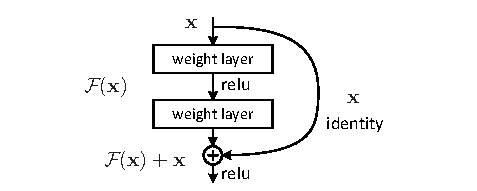
\includegraphics[width=0.48\textwidth]{block}
\caption{An example of a building block in the proposed framework. The rectangle in solid and
dotted lines denote convolution and deconvolution respectively. $\oplus$ denotes element-wise sum of feature maps.}
\label{fig4}
\end{figure}

Instead of directly learning the mappings from the input $X$ to the output $Y$, we would like the network
to fit the residual~\cite{DBLP:journals/corr/HeZRS15} of the problem, which is denoted as $\mathcal{F}(X)=Y-X$.
Such a learning strategy is applied to inner blocks of the encoding-decoding network to make training more
effective. Skip connections are passed every two convolutional layers to their mirrored deconvolutional
layers. Other configurations are possible and our experiments show that this configuration already works
very well. Using such shortcuts makes the network easier to be trained and gains restoration performance
by increasing the network depth.




\subsection{Training}

In general, there are three types of layers in our network: convolution, deconvolution
and element-wise sum. Each layer is followed by a Rectified Linear Unit (ReLU)
~\cite{DBLP:conf/icml/NairH10}. Let $X$ be the input, the convolutional and
deconvolutional layers are expressed as:
\begin{equation}
F(X) = \max(0,W_k * X + B_k),
\end{equation}
where $W_k$ and $B_k$ represent the filters and biases, and $*$ denotes either
convolution or deconvolution operation for the convenience of formulation.
For element-wise sum layer, the output is the element-wise sum of two inputs
of the same size, followed by the ReLU activation:
\begin{equation}
F(X_1,X_2) = \max(0, X_1 + X_2)
\end{equation}

Learning the end-to-end mapping from corrupted images to clean images needs to
estimate the weights $\Theta$ represented by the convolutional and deconvolutional
kernels. Specifically, given a collection of $N$ training sample pairs $\{X^i,Y^i\}$,
where $X^i$ is a noisy image and $Y^i$ is the clean version as the groundtruth.
We minimize the following Mean Squared Error (MSE):
\begin{equation}
  \mathcal{L}(\Theta) = \frac{1}{N}\sum_{i=1}^{N}\|\mathcal{F}(X^i;\Theta)-Y^i\|_F^2.
\label{eq1}
\end{equation}

Traditionally, a  network can learn the mapping from the corrupted image to the clean version
directly. However, our network learns for the additive corruption from the input since there
is a skip connection between the input and the output of the network.
%
%
%
We found that optimizing for the corruption converges better than
optimizing for the clean image. In the extreme case, if the input is a clean image, it would be easier
to push the network to be zero mapping (learning the corruption) than to fit an identity
mapping (learning the clean image) with a stack of nonlinear layers.

We implement and train our network using Caffe~\cite{jia2014caffe}. Empirically, we find
that using Adam~\cite{DBLP:journals/corr/KingmaB14} with base learning rate of $10^{-4}$ for
training converges faster than traditional stochastic gradient descent (SGD). The base
learning rate for all layers are the same, different from ~\cite{DBLP:journals/pami/DongLHT16,
DBLP:conf/nips/JainS08}, in which a smaller learning rate is set for the last layer.
This  is not necessary in our network. Specifically, gradients with respect to the
parameters of $i$th layer is firstly computed as:
\begin{equation}
g = \nabla_{\theta_i}\mathcal{L}(\theta_i).
\end{equation}
Then, the two momentum vectors are computed as:
\begin{equation}
m = \beta_1m + (1 - \beta_1)g,\quad v = \beta_2v + (1-\beta_2)g^2.
\end{equation}
The update rule is:
\begin{equation}
\alpha = \alpha\sqrt{1-\beta_2^t}/(1-\beta_1^t), \quad \theta_i=\theta_i-\alpha m/(\sqrt{v}+\epsilon).
\end{equation}
$\beta_1$, $\beta_2$ and $\epsilon$ are set as the recommended values in~\cite{DBLP:journals/corr/KingmaB14}.

300 images from the Berkeley Segmentation Dataset (BSD)~\cite{MartinFTM01} are used to
generate image patches as the training set for each image restoration task.
%
%
%




\subsection{Testing}

Although trained on local patches, our network can perform restoration on images of arbitrary sizes.
Given a testing image, one can simply go forward through the network, which is already able to
 outperform existing methods. To achieve even better results, we propose
to process a corrupted image on multiple orientations. Different from segmentation, the
filter kernels in our network only eliminate the corruptions, which is usually not sensitive
to the orientation of image contents in low level restoration tasks. Therefore, we can rotate
and mirror flip the kernels and perform forward multiple times, and then average the output to
achieve an ensemble of multiple tests. We see that this can lead to slightly better performance.

% \input{implementation}
\section{Experiments}
\vspace{-0.05in}

In this section, we conduct a series of experiments to evaluate our model. 
To explore whether the model learns to perform the spatial inference necessary for answering visual questions that explicitly require spatial reasoning, we design a set of experiments using synthetic visual question/answer data in Sec.~\ref{sec:synthetic1}. The experimental results of our model in standard datasets (DAQUAR~\cite{DBLP:journals/corr/MalinowskiF14} and VQA~\cite{DBLP:journals/corr/AntolALMBZP15} datasets) are reported in Sec.~\ref{sec:expstandard}.

%%%%%%%%%%%%%%%%%%%%%%%%%%%%%%%%%%%%%%%%%%%%%%%%%%%%%%%%%%%%%%%%%%%%%%%%%%%%%%%%%%%%%%%%%%%%%%%%%%%
\subsection{Exploring Attention on Synthetic Data}\label{sec:synthetic1}
%Several public datasets are available, however, 
The questions in the public VQA datasets are quite varied and difficult and often require common sense knowledge to answer (e.g., ``Does this man have 20/20 vision?'' about a person wearing glasses). Furthermore, past work~\cite{malinowski2015ask,DBLP:journals/corr/RenKZ15} showed that the question text alone (no image) is a very strong predictor of the answer.
Therefore, before evaluating on standard datasets, we would first like to
understand how the proposed model uses spatial attention to answer simple visual questions where the answer cannot be predicted from question alone. 
Our visualization demonstrates that the attention mechanism does learn to attend to objects and gather evidence via certain inference rules. 

%%%%%%%%%%% figure
\begin{figure*}[!t]
  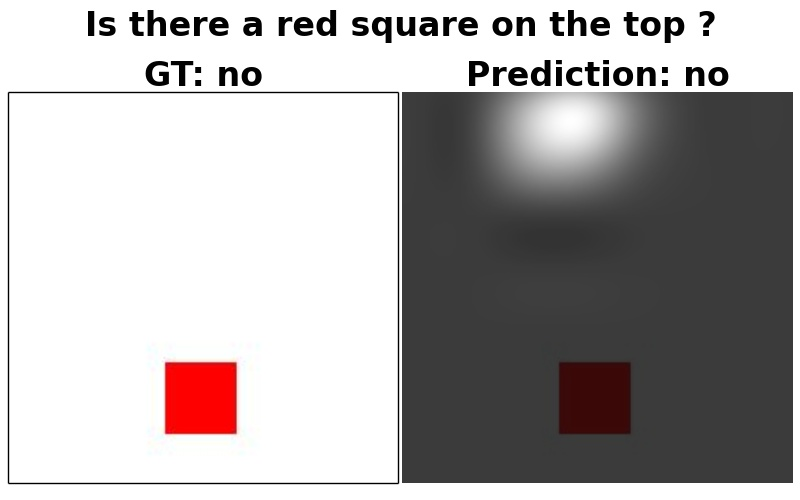
\includegraphics[width=0.242\textwidth]{figures/rule1_im_30075_219_top.JPEG}
  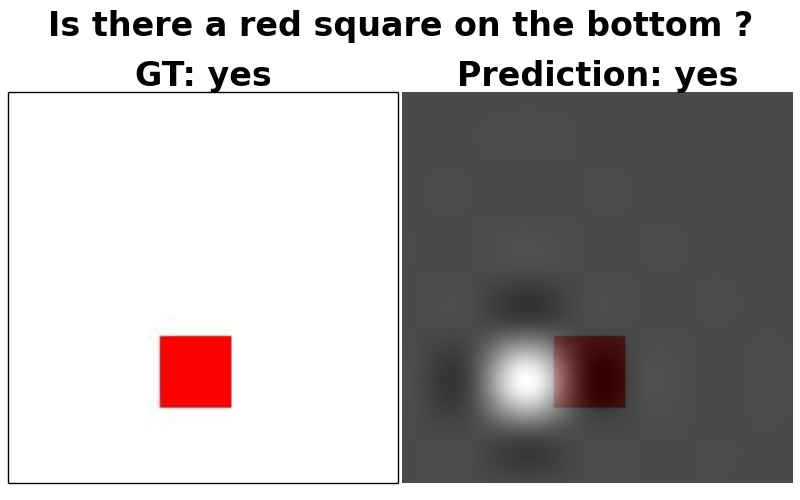
\includegraphics[width=0.242\textwidth]{figures/rule1_im_31186_4441_bottom.JPEG}
  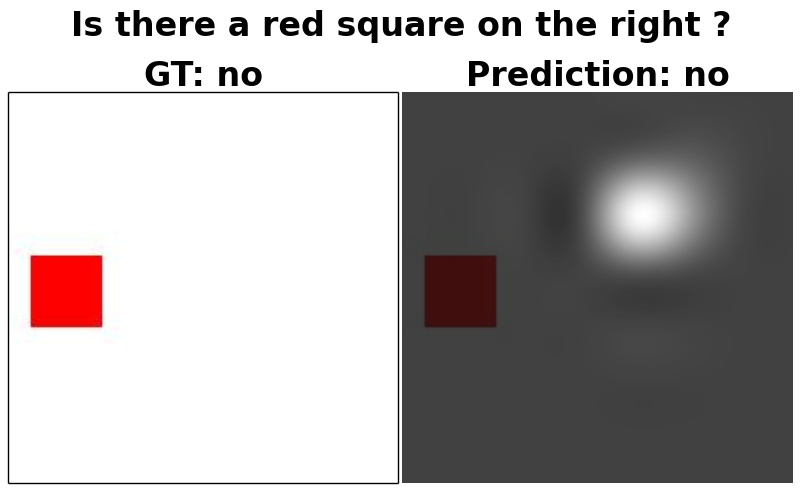
\includegraphics[width=0.242\textwidth]{figures/rule1_im_31189_690_right.JPEG}
  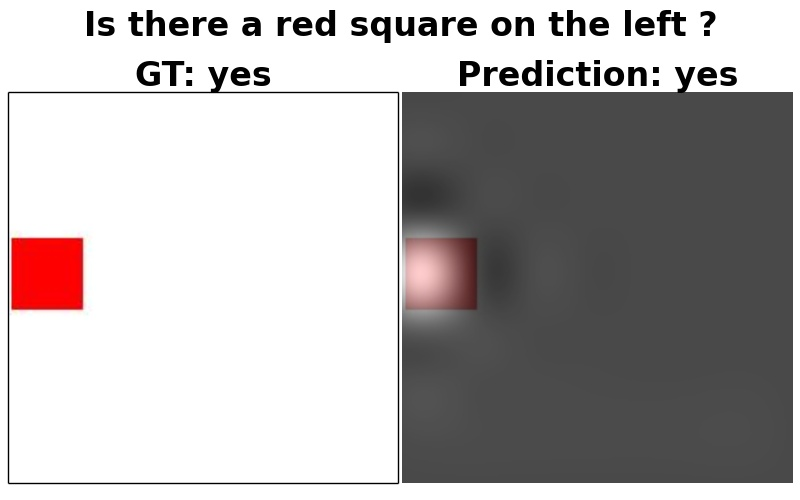
\includegraphics[width=0.242\textwidth]{figures/rule1_im_31200_4217_left.JPEG}\\
  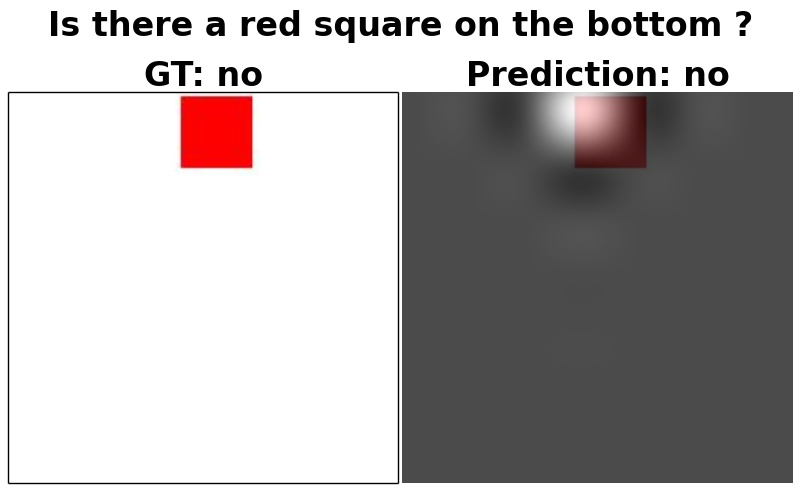
\includegraphics[width=0.242\textwidth]{figures/rule2_im_30004_3495_bottom.JPEG}
  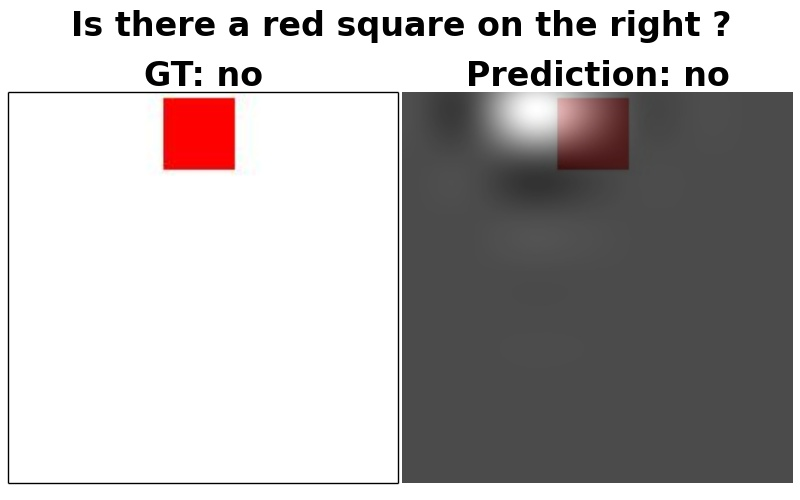
\includegraphics[width=0.242\textwidth]{figures/rule2_im_30036_3165_right.JPEG}
  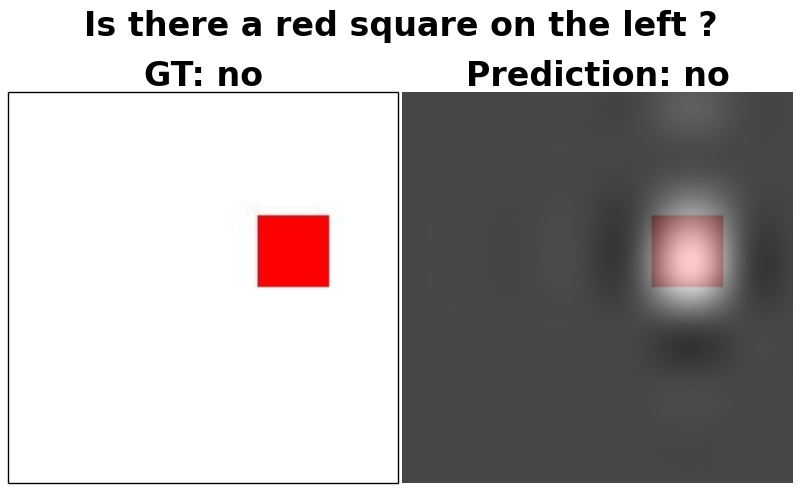
\includegraphics[width=0.242\textwidth]{figures/rule2_im_31185_2199_left.JPEG}
  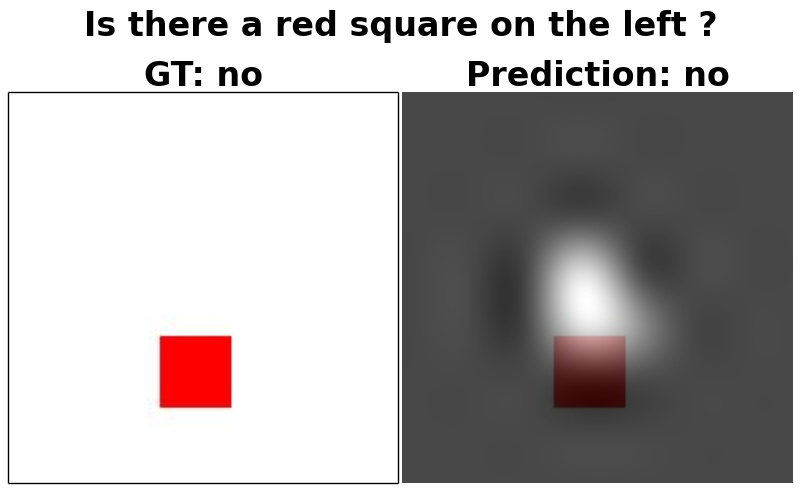
\includegraphics[width=0.242\textwidth]{figures/rule2_im_31186_1310_left.JPEG}
%\includegraphics[width=\textwidth]{figures/onehop_twohop.png}
\vspace{-0.1in}
\caption{\textbf{Absolute position experiment:} for each image and question pair, we show the original image (left) and the attention weights $W_{att}$ (right). 
The attention follows the following rules. The first rule (top row) looks at the position specified in question (top$\mid$bottom$\mid$right$\mid$left), if it contains a square, answer ``yes''; otherwise answer ``no''.
The second rule (bottom row) looks at the region where there is a square, and answers ``yes'' if the question contains that position and ``no'' for the other three positions.}\label{fig:red_square}
\vspace{-0.1in}
\end{figure*}


%%%%%%%%%%%%%%%%%%%%%%%%%%%%%%%%%%%%%%%%%%%%%%%%%%%%%%%%%%%%%%%%%%%%%%%%%%%%%%%%%%%%%%%%%%%%%%%%%%%
\vspace{-0.1in}
\subsubsection{Absolute Position Recognition}\label{sec:absolute}
We investigate whether the model has the ability to recognize the absolute location of the object in the image. We explore this by designing a simple task where an object (a red square) appears in some region of a white-background image, and the question is ``Is there a red square on the [top$\mid$bottom$\mid$left$\mid$right]?'' For each image, we randomly place the square in one of the four regions, and generate the four questions above, together with three ``no'' answers and one ``yes'' answer. The generated data is split into training and testing sets. 

Due to the simplicity of this synthetic dataset, the SMem-VQA one-hop model achieves 100\% test accuracy. However, the baseline model (iBOWIMG)~\cite{zhou2015simple} cannot infer the answer and only obtains accuracy of around 75\%, which is the prior probability of the answer ``no'' in the training set. The SMem-VQA one-hop model is equivalent to the iBOWIMG model if the attention weights in our one-hop model are set equally for each location, since the iBOWIMG model uses the mean pool of the convolutional feature ($inception\_5b/output$) in GoogLeNet that we use in SMem-VQA model. 
We check the visualization of the attention weights and find that the relationship between the high attention position and the answer can be expressed by logical expressions.
We show the attention weights of several typical examples in Fig.~\ref{fig:red_square} which reflect two logic rules:
1)~Look at the position specified in question (top$\mid$bottom$\mid$right$\mid$left), if it contains a square, then answer ``yes''; if it does not contain a square, then answer ``no''.
2)~Look at the region where there is a square, then answer ``yes'' for the question about that position and ``no'' for the questions about the other three positions.

In the iBOWIMG model, the mean-pooled GoogLeNet visual features lose spatial information and thus cannot distinguish images with a square in different positions. On the contrary, our SMem-VQA model can pay high attention to different regions according to the question, and generate an answer based on the selected region, using some learned inference rules.
This experiment demonstrates that the attention mechanism in our model is able to make absolute spatial location inference based on the spatial attention. 


%%%%%%%%%%% figure
\begin{figure*}[t]
  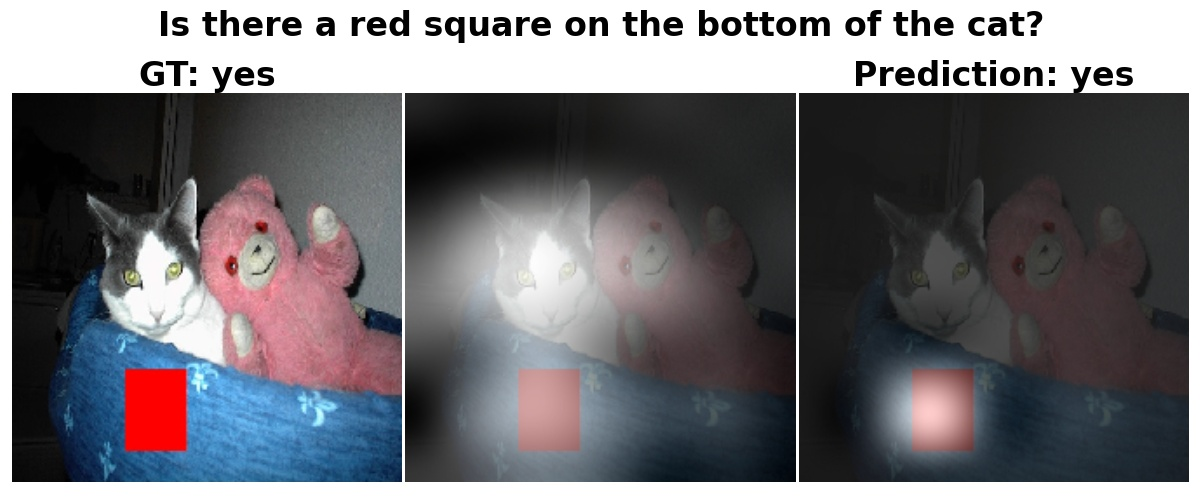
\includegraphics[width=0.325\textwidth]{figures/bottom_COCO_val2014_000000167602_bottom.jpg}
  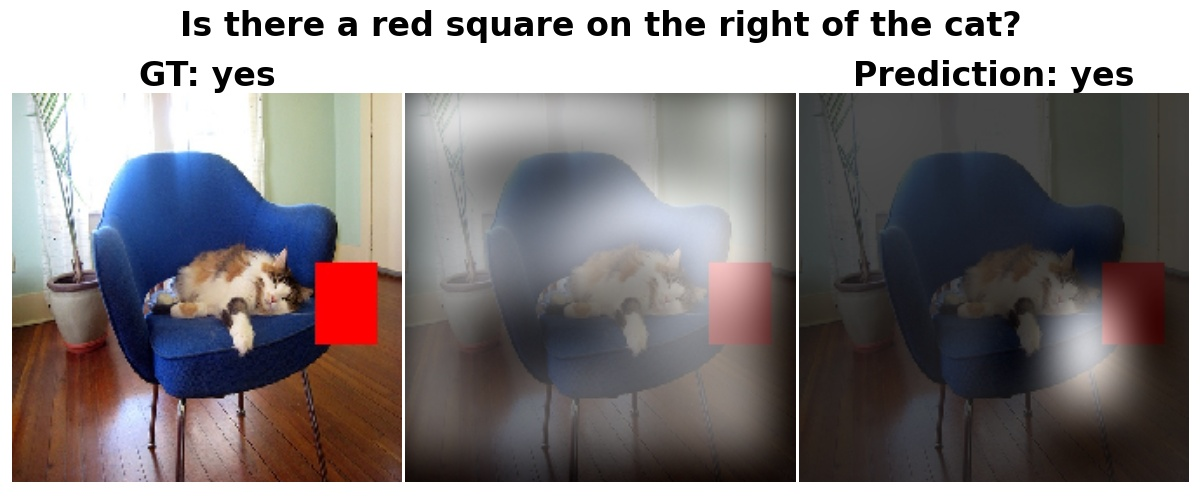
\includegraphics[width=0.325\textwidth]{figures/right_COCO_val2014_0000002988_right.jpg}
  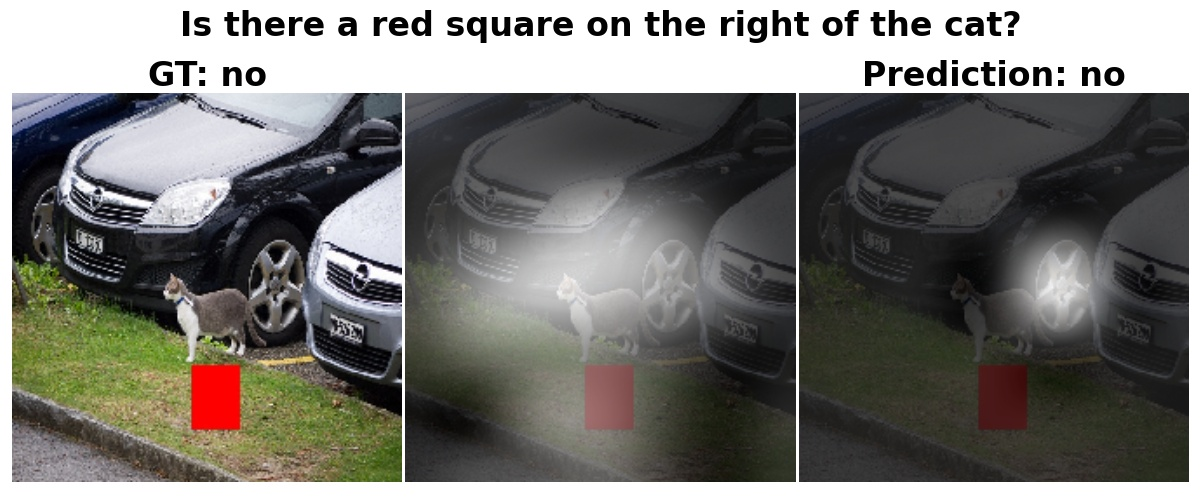
\includegraphics[width=0.325\textwidth]{figures/right_COCO_val2014_000000172330_bottom.jpg}\\
  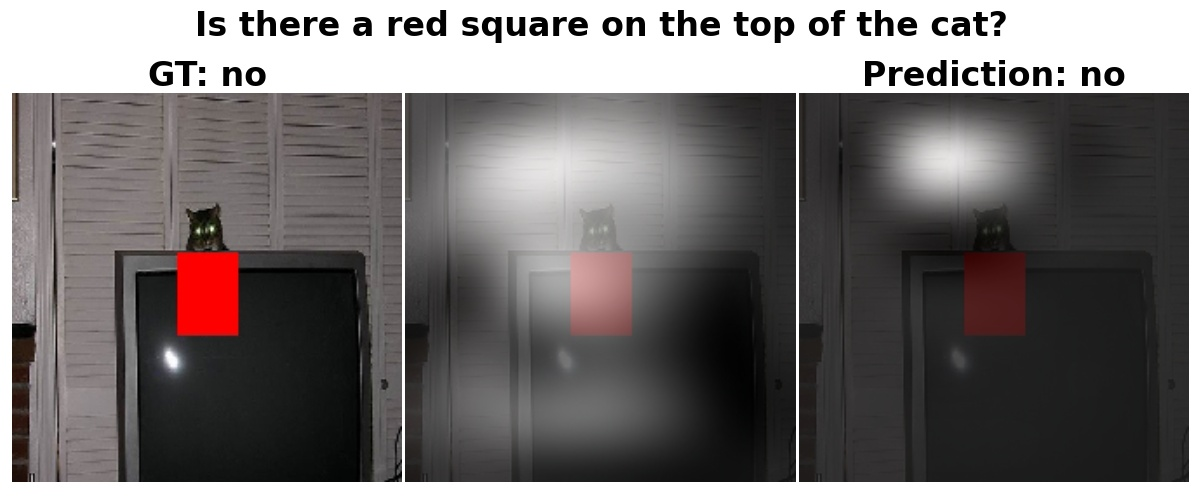
\includegraphics[width=0.325\textwidth]{figures/top_COCO_val2014_00000010694_bottom}
  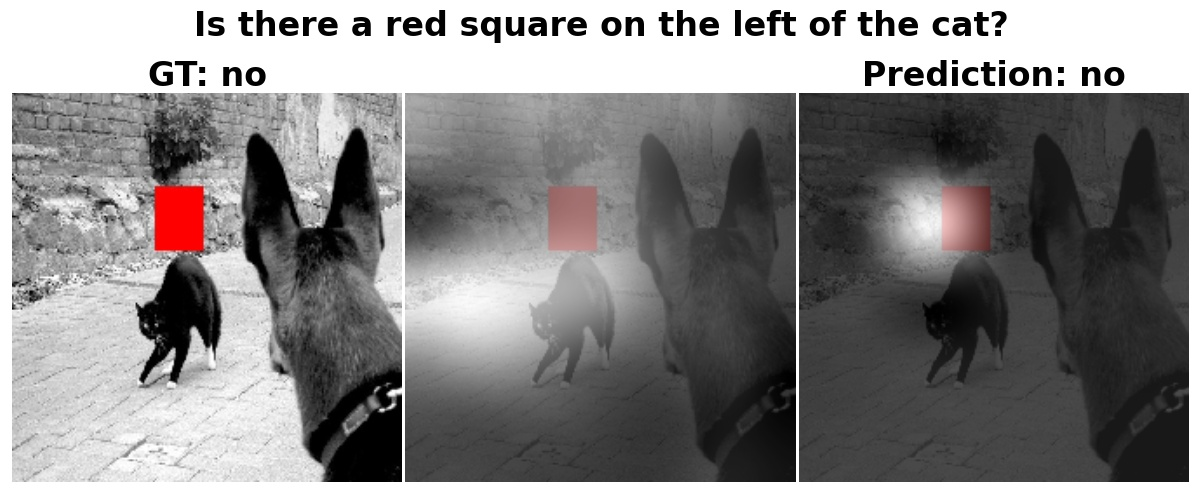
\includegraphics[width=0.325\textwidth]{figures/left_COCO_val2014_000000201918_top.jpg}
  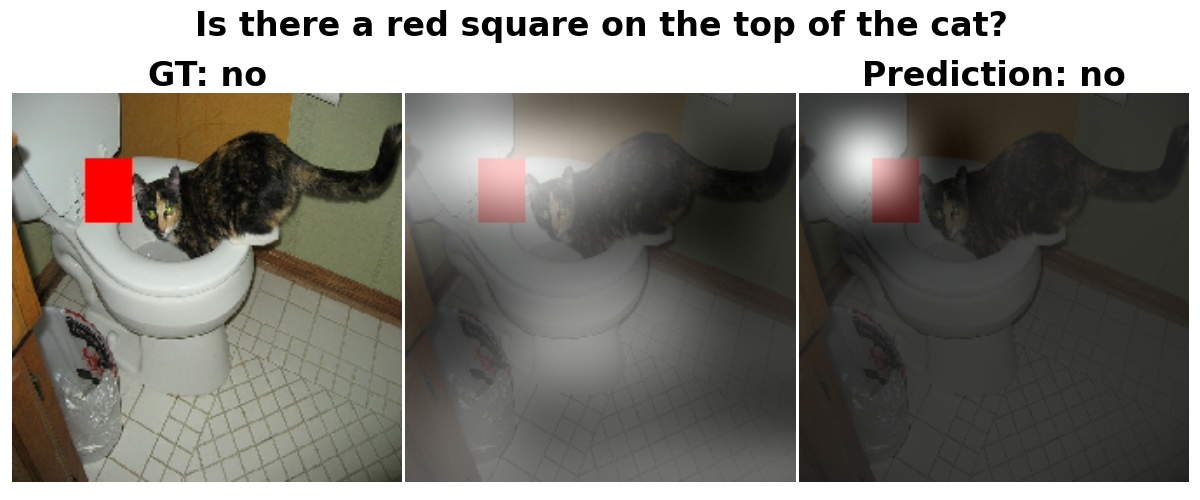
\includegraphics[width=0.325\textwidth]{figures/top_COCO_val2014_000000218924_left.jpg}
\vspace{-0.05in}
\caption{\textbf{Relative position experiment:}
for each image and question pair, we show the original image (left), the evidence embedding $W_E$ of the convolutional layer (middle) and the attention weights $W_{att}$ (right). The evidence embedding $W_E$ has high activations on both cat and red square. 
The attention weights follow similar inference rules as in Fig.~\ref{fig:red_square}, with the difference that the attention position is around the cat.
%Rule#1: (top row) look at the specified position (top/bottom/right/left), if it contains a square, answer "yes"; otherwise answer "no".
%Rule#2: (bottom row) look at the region where there is a square, answer "yes" if the question contains that position and "no" if it contains one of the other three positions.
}\label{fig:cat_square}
\vspace{-0.2in}
\end{figure*}


%%%%%%%%%%%%%%%%%%%%%%%%%%%%%%%%%%%%%%%%%%%%%%%%%%%%%%%%%%%%%%%%%%%%%%%%%%%%%%%%%%%%%%%%%%%%%%%%%%%
\vspace{-0.1in}
\subsubsection{Relative Position Recognition}
In order to check whether the model has the ability to infer the  position of one object \textit{relative} to another object,
we collect all the cat images from the MS COCO Detection dataset~\cite{lin2014microsoft}, and add a red square on the [top$\mid$bottom$\mid$left$\mid$right] of the bounding box of the cat in the images.
For each generated image, we create four questions, ``Is there a red square on the [top$\mid$bottom$\mid$left$\mid$right] of the cat?'' together with three ``no'' answers and one ``yes'' answer. 
We select 2639 training cat images and 1395 testing cat images from MS COCO Detection dataset. 

Our SMem-VQA one-hop model achieves 96\% test accuracy on this synthetic task, while the baseline model (iBOWIMG) accuracy is around 75\%.
We also check that another simple baseline that predicts the answer based on the absolute position of the square in the image gets around 70\% accuracy. 
We visualize the evidence embedding $W_E$ features and the attention weights $W_{att}$ of several typical examples in Fig.~\ref{fig:cat_square}.
The evidence embedding $W_E$ has high activations on the cat and the red square, while the attention weights pay high attention to certain locations around the cat.
We can analyze the attention in the correctly predicted examples using the same rules as in absolute position recognition experiment. 
These rules still work, but the position is relative to the cat object:
1)~Check the specified position relative to the cat, if it finds the square, then answer ``yes'', otherwise ``no''; 2)~Find the square, then answer ``yes'' for the specified position, and answer ``no'' for the other positions around the cat.
We also check the images where our model makes mistakes, and find that the mistakes mainly occur in images with more than one cats. The red square appears near only one of the cats in the image, but our model might make mistakes by focusing on the other cats.
We conclude that our SMem-VQA model can infer the relative spatial position based on the spatial attention around the specified object, which can also be represented by some logical inference rules. 



%%%%%%%%%%%%%%%%%%%%%%%%%%%%%%%%%%%%%%%%%%%%%%%%%%%%%%%%%%%%%%%%%%%%%%%%%%%%%%%%%%%%%%%%%%%%%%%%%%%
%%%%%%%%%%%%%% table
\begin{table}[!t]
\centering
\caption{Accuracy results on the DAQUAR dataset (in percentage).}
\small
 \begin{tabular}{l || c c c} 
 \hline
 ~ & DAQUAR\\ \hline
 Multi-World~\cite{DBLP:journals/corr/MalinowskiF14} & 12.73 \\ %\hline
 Neural-Image-QA~\cite{malinowski2015ask} & 29.27  \\ %\hline
 Question LSTM~\cite{malinowski2015ask} & 32.32 \\ %\hline
 VIS+LSTM~\cite{DBLP:journals/corr/RenKZ15} & 34.41 \\ %\hline
 Question BOW~\cite{DBLP:journals/corr/RenKZ15} & 32.67 \\ %\hline
 IMG+BOW~\cite{DBLP:journals/corr/RenKZ15} & 34.17 \\ \hline
 %2-VIS+BLSTM ~\cite{DBLP:journals/corr/RenKZ15} &  - & 35.78  & -\\ \hline \hline
 %Question One-Hop & 53.37 & 36.03 & - \\ %\hline   
 SMem-VQA One-Hop & 36.03 \\ %\hline   
 SMem-VQA Two-Hop & \bf{40.07} \\ \hline 
 %one dimension convolution hierarchy model\cite{ma2015learning} &  - & 0.3933 \cite{ma2015learning} & - \\ \hline
 \end{tabular}
\label{fig:baseline}
\vspace{-0.2in}
\end{table}


\subsection{Experiments on Standard Datasets}\label{sec:expstandard}
%\vspace{-0.08in}
\subsubsection{Results on DAQUAR}
The DAQUAR dataset is a relatively small dataset which builds on the NYU Depth Dataset V2~\cite{Silberman:ECCV12}. We use the reduced DAQUAR dataset~\cite{DBLP:journals/corr/MalinowskiF14}. The evaluation metric for this dataset is 0-1 accuracy. 
The embedding dimension is 512 for our models running on the DAQUAR dataset. 
We use several reported models on DAQUAR as baselines, which are listed below:\\
%\noindent
{$\bullet$} {\bf{Multi-World}}~\cite{DBLP:journals/corr/MalinowskiF14}: an approach based on handcrafted features using a semantic parse of the question and scene analysis of the image combined in a latent-world Bayesian framework.\\ 
{$\bullet$} {\bf{Neural-Image-QA}}~\cite{malinowski2015ask}: uses an LSTM to encode the question and then decode the hidden information into the answer. The image CNN feature vector is shown at each time step of the encoding phase.\\
{$\bullet$} {\bf{Question LSTM}}~\cite{malinowski2015ask}: only shows the question to the LSTM to predict the answer without any image information.\\
{$\bullet$} {\bf{VIS+LSTM}}~\cite{DBLP:journals/corr/RenKZ15}: similar to Neural-Image-QA, but only shows the image features to the LSTM at the first time step, and the question in the remaining time steps to predict the answer.\\
{$\bullet$} {\bf{Question BOW}}~\cite{DBLP:journals/corr/RenKZ15}: only uses the BOW question representation and a single hidden layer neural network to predict the answer, without any image features.\\
{$\bullet$} {\bf{IMG+BOW}}~\cite{DBLP:journals/corr/RenKZ15}: concatenates the BOW question representation with image features, and then uses a single hidden layer neural network to predict the answer. This model is similar to the iBOWIMG baseline model in~\cite{zhou2015simple}.

Results of our SMem-VQA model on the DAQUAR dataset and the baseline model results reported in previous work are shown in Tab.~\ref{fig:baseline}. 
From the DAQUAR result in Tab.~\ref{fig:baseline}, we see that models based on deep features significantly outperform the Multi-World approach based on hand-crafted features. Modeling the question only with either the LSTM model or Question BOW model does equally well in comparison, indicating the the question text contains important prior information for predicting the answer. Also, on this dataset, the VIS+LSTM model achieves better accuracy than Neural-Image-QA model; the former shows the image only at the first timestep of the LSTM, while the latter does so at each timestep. In comparison, both our One-Hop model and Two-Hop spatial attention models outperform the IMG+BOW, as well as the other baseline models.
A major advantage of our model is the ability to visualize the inference process in the deep network. To illustrate this, two attention weights visualization examples in SMem-VQA One-Hop and Two-Hop models on DAQUAR dataset are shown in Fig.~\ref{fig:2hopVQA} (bottom row).



%%%%%%%%%%% figure
\begin{figure*}[t]
%  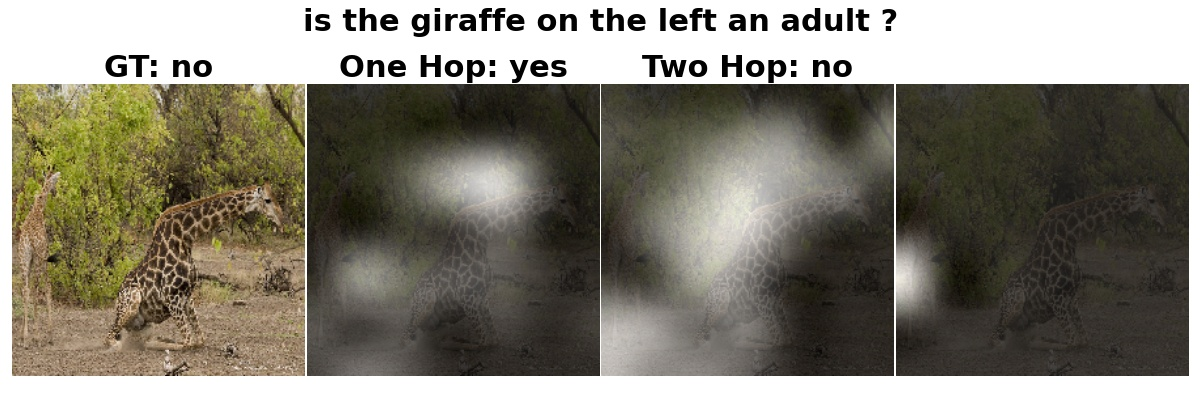
\includegraphics[width=0.5\textwidth]{figures/VQA-DAQUAR_One-Hop_Two-Hop/COCO_val2014_000000014271.jpg}
%  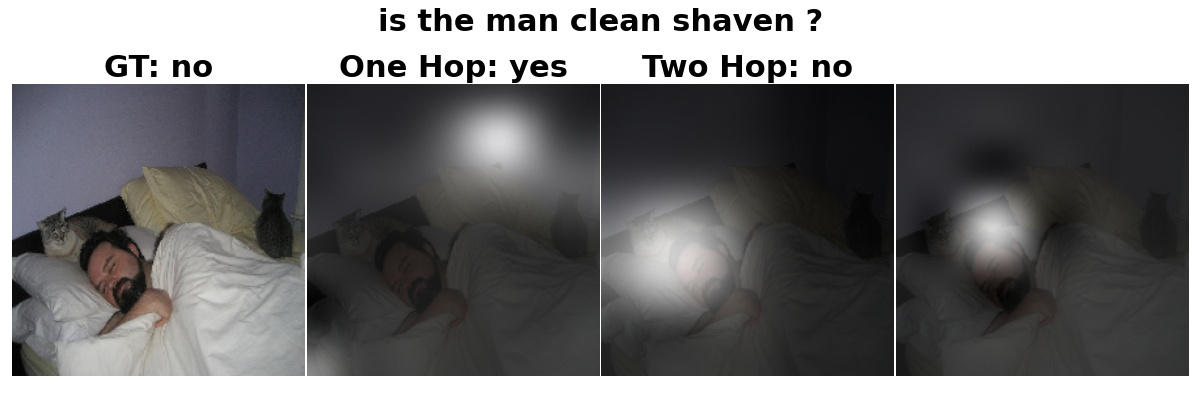
\includegraphics[width=0.5\textwidth]{figures/VQA-DAQUAR_One-Hop_Two-Hop/COCO_val2014_000000012085.jpg}\\
  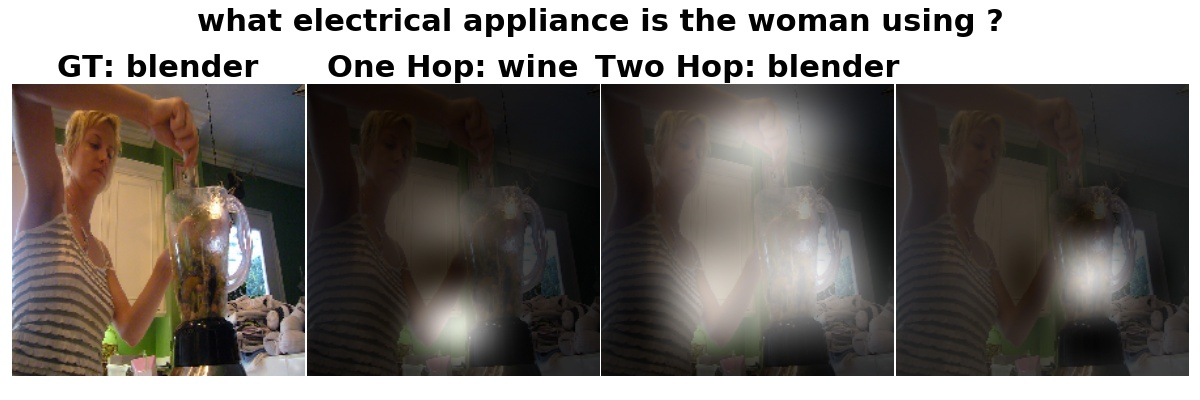
\includegraphics[width=0.5\textwidth]{figures/VQA-DAQUAR_One-Hop_Two-Hop/CO_train2014_000000575060_5750602.jpg}
  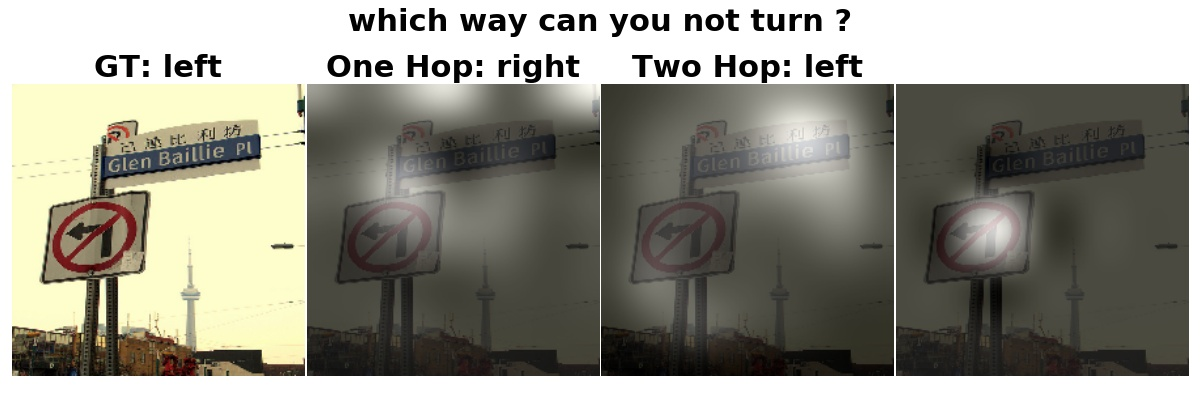
\includegraphics[width=0.5\textwidth]{figures/VQA-DAQUAR_One-Hop_Two-Hop/CO_train2014_000000222383_2223830.jpg}\\
  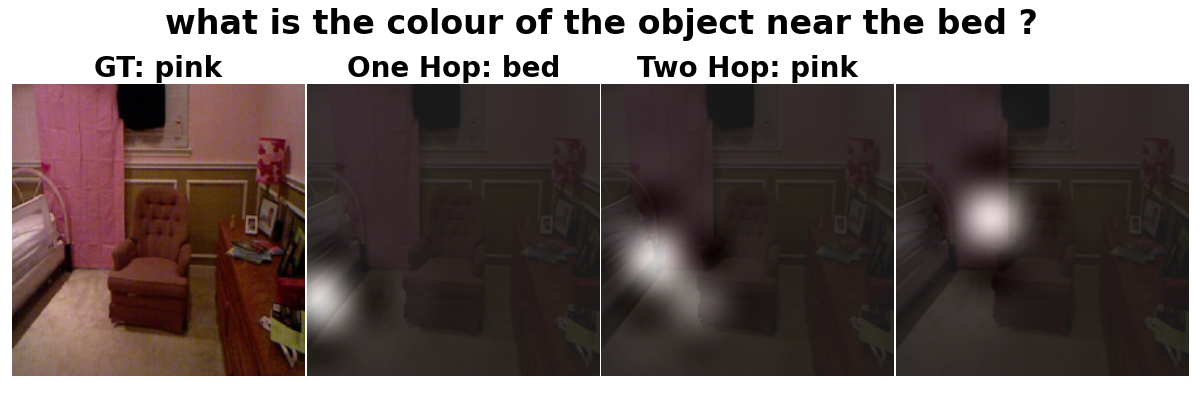
\includegraphics[width=0.5\textwidth]{figures/VQA-DAQUAR_One-Hop_Two-Hop/image1183.png}
  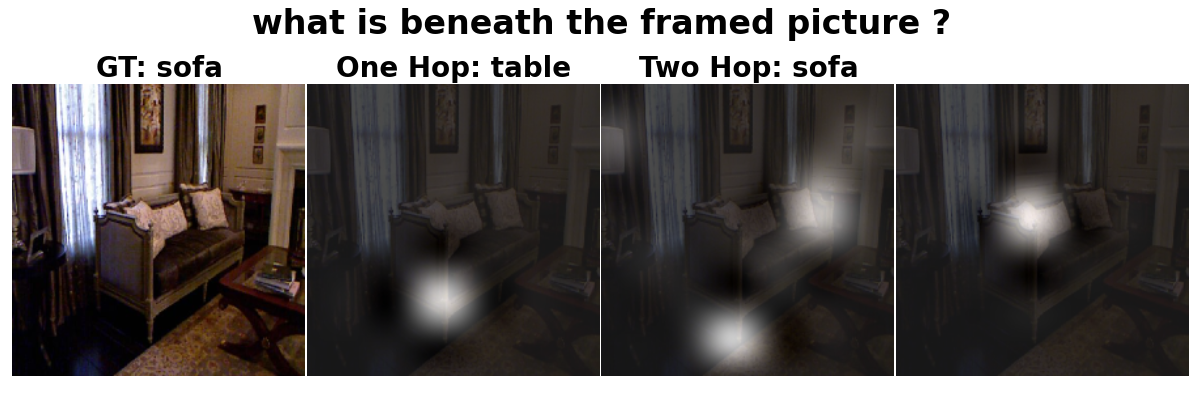
\includegraphics[width=0.5\textwidth]{figures/VQA-DAQUAR_One-Hop_Two-Hop/image1444.png}
\vspace{-0.25in}
\caption{Visualization of the spatial attention weights in the SMem-VQA One-Hop and Two-Hop models on VQA (top row) and DAQUAR (bottom row) datasets. For each image and question pair, we show the original image, the attention weights $W_{att}$ of the One-Hop model, and the two attention weights $W_{att}$ and $W_{att2}$ of the Two-Hop model in order.}\label{fig:2hopVQA}
\vspace{-0.15in}
\end{figure*}
% \vspace{-0.1in}
\subsubsection{Results on VQA}

The VQA dataset is a recent large dataset based on MS COCO~\cite{lin2014microsoft}. We use the full release (V1.0) open-ended dataset, which contains a train set and a val set. Following standard practice, we choose the top 1000 answers in train and val sets as possible prediction answers, and only keep the examples whose answers belong to these 1000 answers as training data. The question vocabulary size is 7477 with the word frequency of at least three.
Because of the larger training size, the embedding dimension is 1000 on the VQA dataset.
We report the test-dev and test-standard results from the VQA evaluation server.
The server evaluation uses the evaluation metric introduced by~\cite{DBLP:journals/corr/AntolALMBZP15}, which gives partial credit to certain synonym answers:
%\begin{equation}
%Acc({\color{red}ans}) = \min\left\{ \frac{\text{\# human that said }{\color{red} ans}}{3},1\right\}
%$Acc({ans}) = \min\left\{ \frac{\text{\# humans that said }{ans}}{3},1\right\}$.
$Acc({ans}) = \min\left\{ (\text{\# humans that said }{ans})/3,1\right\}$.
%\end{equation}


For the attention models, we do not mirror the input image when using the CNN to extract convolutional features, since this might cause confusion about the spatial locations of objects in the input image.
%The input image size for CNN is $224 \times 224$.
The optimization algorithm used is stochastic gradient descent (SGD) with a minibatch of size 50 and momentum of 0.9.
The base learning rate is set to be 0.01 which is halved every six epoches. Regularization, dropout and L2 norm are cross-validated and used. 


%%%%%%%%%%%%%% another candidate table with test-standard
\begin{table}[!t]
\centering
\caption{Test-dev and test-standard results on the Open-Ended VQA dataset (in percentage). Models with ${}^\ast$ use external training data in addition to the VQA dataset.}
\scriptsize
 \begin{tabular}{l || c c c c || c c c c} 
 \hline
 ~ & \multicolumn{4}{c||}{test-dev}  & \multicolumn{4}{c}{test-standard}\\ 
 ~ & \bf{Overall}  & yes/no  & number  & others & \bf{Overall}  & yes/no  & number  & others\\ \hline
 LSTM Q+I~\cite{DBLP:journals/corr/AntolALMBZP15} & 53.74 & 78.94  & 35.24  & 36.42 & 54.06 & -  & -  & -\\ %\hline
 ACK${}^\ast$~\cite{wu2015ask} & 55.72 & 79.23  & 36.13  & 40.08 & 55.98 & 79.05  & 36.10  & 40.61\\ %\hline
 DPPnet${}^\ast$~\cite{noh2015image} & 57.22 & 80.71  & 37.24  & 41.69 & 57.36 & 80.28  & 36.92  & 42.24\\ %\hline
 iBOWIMG~\cite{zhou2015simple} & 55.72 & 76.55  & 35.03  & 42.62 & 55.89 & 76.76  & 34.98  & 42.62\\ \hline 
 SMem-VQA One-Hop & 56.56 & 78.98 & 35.93  & 42.09 & - & -  & -  & -\\ %\hline   
 SMem-VQA Two-Hop & \textbf{57.99} & \textbf{80.87}  & \textbf{37.32}  & \textbf{43.12} & \textbf{58.24} & \textbf{80.8}  & \textbf{37.53}  & \textbf{43.48}\\ \hline 
 \end{tabular}
\label{fig:baseline2}
\vspace{-0.15in}
\end{table}

For the VQA dataset, we use the simple iBOWIMG model in~\cite{zhou2015simple} as one baseline model, which beats most existing VQA models currently on arxiv.org. We also compare to two models in~\cite{wu2015ask}\cite{noh2015image} which have comparable or better results to the iBOWIMG model. These three baseline models as well the best model in VQA dataset paper~\cite{DBLP:journals/corr/AntolALMBZP15} are listed in the following:\\
%\noindent
{$\bullet$} {\bf{LSTM Q+I}}~\cite{DBLP:journals/corr/AntolALMBZP15}: uses the element-wise multiplication of the LSTM encoding of the question and the image feature vector to predict the answer. This is the best model in the VQA dataset paper.\\
{$\bullet$} {\bf{ACK}}~\cite{wu2015ask}: shows the image attribute features, the generated image caption and relevant external knowledge from knowledge base to the LSTM at the first time step, and the question in the remaining time steps to predict the answer.\\
{$\bullet$} {\bf{DPPnet}}~\cite{noh2015image}: uses the Gated Recurrent Unit (GRU) representation of question to predict certain parameters for a CNN classification network. They pre-train the GRU for question representation on a large-scale text corpus to improve the GRU generalization performance.\\
{$\bullet$} {\bf{iBOWIMG}}~\cite{zhou2015simple}: concatenates the BOW question representation with image feature (GoogLeNet), and uses a softmax classification to predict the answer. 

The overall accuracy and per-answer category accuracy for our SMem-VQA models and the four baseline models on VQA dataset are shown in Tab.~\ref{fig:baseline2}. From the table, we can see that the SMem-VQA One-Hop model obtains slightly better results compared to the iBOWIMG model. However, the SMem-VQA Two-Hop model achieves an improvement of 2.27\% on test-dev and 2.35\% on test-standard compared to the iBOWIMG model, demonstrating the value of spatial attention. The SMem-VQA Two-Hop model also shows best performance in the per-answer category accuracy. 
The SMem-VQA Two-Hop model has slightly better result than the DPPnet model. 
The DPPnet model uses a large-scale text corpus to pre-train the Gated Recurrent Unit (GRU) network for question representation.
Similar pre-training work on extra data to improve model accuracy has been done in~\cite{venugopalan2014translating}.
Considering the fact that our model does not use extra data to pre-train the word embeddings, its results are very competitive.
We also experiment with adding a third hop into our model on the VQA dataset, but the result does not improve further.

The attention weights visualization examples for the SMem-VQA One-Hop and Two-Hop models on the VQA dataset are shown in Fig.~\ref{fig:2hopVQA} (top row). From the visualization, we can see that the two-hop model collects supplementary evidence for inferring the answer, which may be necessary to achieve an improvement on these complicated real-world datasets. We also visualize the fine-grained alignment in the first hop of our SMem-VQA Two-Hop model in Fig.~\ref{fig:VQA_hop1Atten_wordAtten}. 
%through visualizing the attention weights and the correlation value vector from the correlation matrix $C$ for the location with highest attention weight
The correlation vector values (blue bars) measure the correlation between image regions and each word vector in the question. Higher values indicate stronger correlation of that particular word with the specific location's image features. We observe that the fine-grained visual evidence collected using each local word vector, together with the global visual evidence from the whole question, complement each other to infer the correct answer for the given image and question, as shown in Fig.~\ref{fig:concept}.


%%%%%%%%%%% figure
\begin{figure*}[t]
  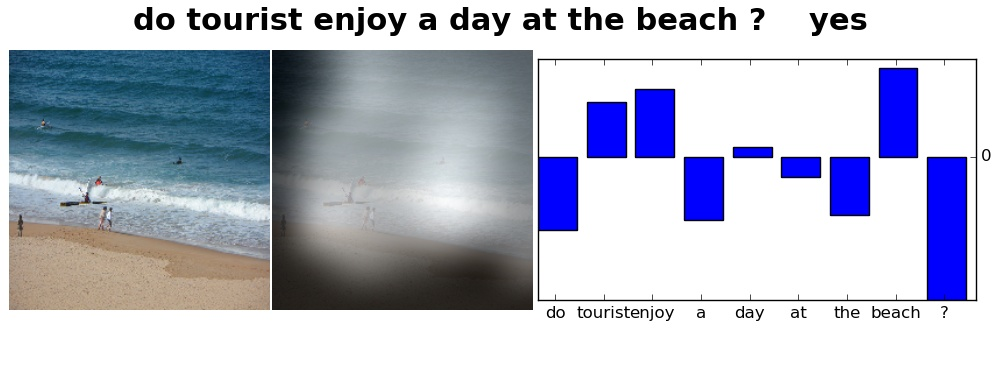
\includegraphics[width=0.5\textwidth]{figures/word_atten/COCO_val2014_000000540932_5409320.jpg}
  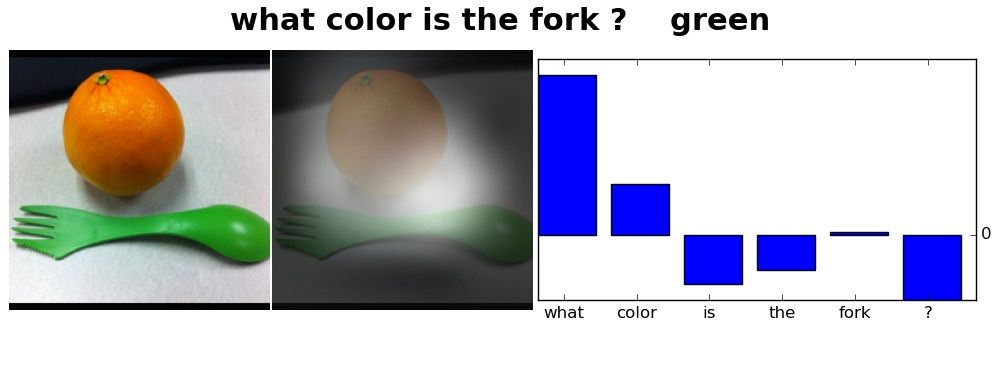
\includegraphics[width=0.5\textwidth]{figures/word_atten/COCO_val2014_000000563730_5637302.jpg}\\
  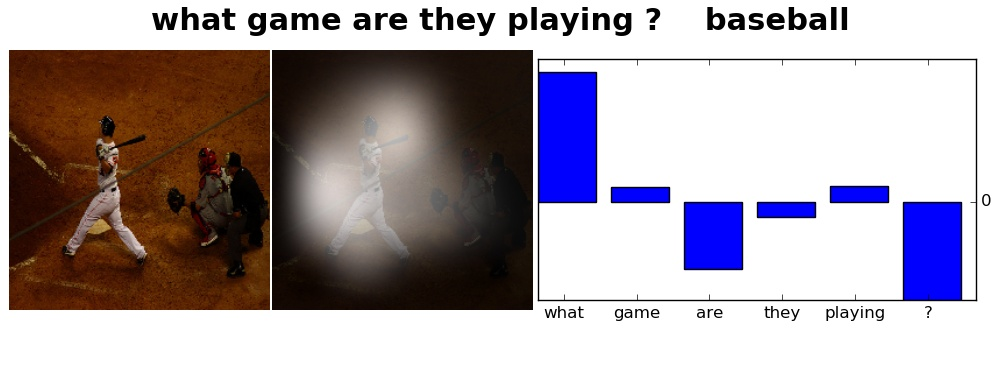
\includegraphics[width=0.5\textwidth]{figures/word_atten/COCO_val2014_000000576875_5768752.jpg}
  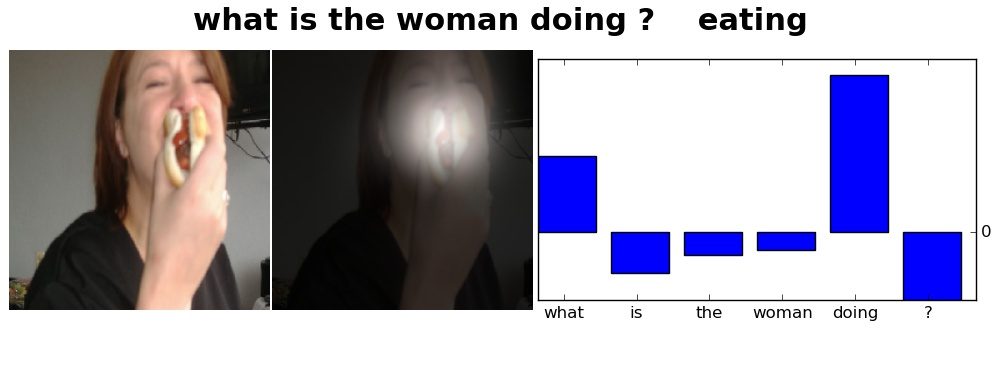
\includegraphics[width=0.5\textwidth]{figures/word_atten/COCO_val2014_000000567340_5673401.jpg}
\vspace{-0.3in}
\caption{
Visualization of the original image (left), the spatial attention weights $W_{att}$ in the first hop (middle) and one correlation vector from the correlation matrix $C$ for the location with highest attention weight in the SMem-VQA Two-Hop model on the VQA dataset.
Higher values in the correlation  vector indicate  stronger correlation of that word with the chosen location's image features.}
\label{fig:VQA_hop1Atten_wordAtten}
\vspace{-0.15in}
\end{figure*}




 






\label{sec:conclusion}
We introduce a novel neural network architecture, the Synchronized Spectral CNN (SyncSpecCNN), for semantic annotation on 3D shape graphs. To share coefficients and conduct multi-scale analysis in different parts of a single shape graph, we introduce a spectral parametrization of dilated convolutional kernels. To allow parameter sharing across related but different shapes that may be represented by very different graphs, we introduce a spectral transformer network to synchronize different spectral domains. The effectiveness of different components in our network is validated through extensive experiments. Jointly these contributions lead to state-of-the-art performance on various semantic annotation tasks including 3D shape part segmentation and 3D keypoint prediction.
\section{Acknowledgment}
This work is partly supported by the Air Force Office of Scientific Research (AFOSR) under the Dynamic Data-Driven Application Systems Program, NSF 1763523, 1747778, 1733843 and 1703883 Awards.

\clearpage

\bibliographystyle{splncs04}
\bibliography{egbib}
\end{document}
